\documentclass[11pt]{article}
\usepackage[T1]{fontenc}
\usepackage{lmodern,microtype}
\usepackage[margin=1in]{geometry}
\usepackage{amsmath,amssymb,amsthm,mathtools,mathrsfs}
\usepackage{booktabs,array,tikz,xcolor}
\PassOptionsToPackage{hyphens}{url}
\usepackage[colorlinks=true,linkcolor=black,citecolor=black,urlcolor=blue]{hyperref}
\hypersetup{pdftitle={Area-controlled end replacement and the Bondi-Penrose inequality in the CKS class},pdfauthor={OpenAI}}
\pdfinfoomitdate=1
\pdftrailerid{}
\pdfsuppressptexinfo=15
\ifdefined\pdfglyphtounicode
  \pdfglyphtounicode{tfm:lmex10/parenleftbig}{0028}
  \pdfglyphtounicode{tfm:lmex10/parenrightbig}{0029}
  \pdfglyphtounicode{tfm:lmex10/parenleftbigg}{0028}
  \pdfglyphtounicode{tfm:lmex10/parenrightbigg}{0029}
  \pdfglyphtounicode{tfm:lmex10/bracketleftbigg}{005B}
  \pdfglyphtounicode{tfm:lmex10/bracketrightbigg}{005D}
  \pdfglyphtounicode{tfm:lmex10/vextendsingle}{23D0}
  \pdfglyphtounicode{tfm:lmex10/summationtext}{2211}
  \pdfglyphtounicode{tfm:lmex10/summationdisplay}{2211}
  \pdfglyphtounicode{tfm:lmex10/integraltext}{222B}
  \pdfglyphtounicode{tfm:lmex10/integraldisplay}{222B}
  \pdfglyphtounicode{tfm:lmex10/hatwide}{02C6}
  \pdfglyphtounicode{tfm:lmex10/radicalbig}{221A}
  \pdfglyphtounicode{tfm:lmex10/radicalBig}{221A}
  \pdfglyphtounicode{tfm:lmex10/radicalBigg}{221A}
\fi
\numberwithin{equation}{section}
\newtheorem{theorem}{Theorem}[section]
\newtheorem{proposition}[theorem]{Proposition}
\newtheorem{lemma}[theorem]{Lemma}
\newtheorem{corollary}[theorem]{Corollary}
\theoremstyle{definition}
\newtheorem{assumption}[theorem]{Assumption}
\theoremstyle{remark}
\newtheorem{remark}[theorem]{Remark}
\DeclareMathOperator{\tr}{tr}
\DeclareMathOperator{\diver}{div}
\newcommand{\TF}{\mathrm{TF}}
\newcommand{\R}{\mathbb R}
\newcommand{\Sph}{\mathbb S^2}
\newcommand{\avg}[1]{\frac{1}{4\pi}\int_{\Sph}#1\,\mathrm dA_\sigma}
\setlength{\emergencystretch}{2em}
\title{Area-controlled end replacement and the Bondi--Penrose inequality in the CKS class}
\author{OpenAI}
\date{September 27, 2026}
\begin{document}
\maketitle
\begin{abstract}
We replace a three-dimensional Cha--Khuri--Sakovich hyperboloidal end
by an asymptotically flat end while preserving the dominant energy
condition and each fixed compact interior. For strictly future-timelike
CKS initial-data charge, the replacements lose asymptotically no enclosing area
and their ADM masses tend to the invariant Bondi mass. Combining this
construction with the companion numerical spacetime Penrose theorem
yields the sharp Bondi bound for possibly disconnected weakly future
trapped boundaries in this class. Horizon-regular Schwarzschild
exteriors attain equality at every positive mass.
\end{abstract}
\tableofcontents
\section{Replacing the end and retaining the area}\label{sec:introduction}

We ask whether a Cha--Khuri--Sakovich hyperboloidal end can be replaced
by an asymptotically flat end while leaving a prescribed compact
interior unchanged and making the ADM mass approach the Lorentz norm
of the hyperboloidal charge.
For the Penrose inequality, a mass comparison alone is insufficient.
A surface enclosing the inner boundary can travel through the modified
end, so its area must remain controlled wherever the replacement occurs.

We construct replacements that preserve the dominant energy condition
and give a lower metric comparison on the entire exterior. This controls
every enclosing surface at once, including disconnected surfaces and
surfaces touching the original boundary. The construction applies to
the precise asymptotic class of Cha, Khuri and Sakovich
\cite{CKS}. The end replacement is the main geometric result; the sharp
Bondi inequality follows by applying the numerical asymptotically flat
inequality to each completed replacement.

\subsection{The exterior, its charges and its enclosing cuts}
Let $\Omega$ be a connected orientable smooth three-manifold with
nonempty compact smooth boundary $S$. Let $g$ be a smooth Riemannian
metric and $K$ a smooth symmetric covariant two-tensor, both smooth up
to $S$. We require completeness as a metric space with $S$ included,
and exactly one coordinate end with compact complement.
With $G=c=1$ and zero cosmological constant, the constraint densities are
\begin{equation}\label{eq:constraints-definition}
 16\pi\mu=R_g+(\tr_gK)^2-|K|_g^2,
 \qquad 8\pi J=\diver_g\bigl(K-(\tr_gK)g\bigr).
\end{equation}
The dominant energy condition (DEC) is $\mu\geq |J|_g$.
For a two-sided surface with normal $\nu$ pointing into its end side,
write
\[
 H=\diver_{\mathrm{surface}}\nu,\qquad
 \theta_+=H+\tr_{\mathrm{surface}}K,\qquad
 \theta_-=H-\tr_{\mathrm{surface}}K.
\]
Thus a future marginally outer trapped surface has $\theta_+=0$.
Our spacetime convention is
$K(Y,Z)=\overline g(\overline\nabla_Yn_{\mathrm{future}},Z)$;
the future unit hyperboloid in Minkowski space has $K=g$.

An \emph{enclosing cut} is $\Gamma=\partial D$, the intrinsic manifold
boundary of a connected smooth codimension-zero submanifold-with-boundary
$D\subset\Omega$ that is closed in $\Omega$, contains the whole
sufficiently distant end, and has manifold interior in
$\operatorname{int}\Omega$. Its full boundary must be compact, smooth,
embedded and two-sided. Every component and every portion coinciding
with $S$ contributes its area. A cut need not be connected, trapped or
minimal. Set
\begin{equation}\label{eq:area-definition}
 A_{\min,g}(S)=\inf_\Gamma\operatorname{Area}_g(\Gamma).
\end{equation}
Taking $D=\Omega$ shows that the class includes $S$ itself. We neither
assume attainment of the infimum nor identify it with
$\operatorname{Area}_g(S)$. This distinction matters for the Penrose
inequality: Ben-Dov's spherical example violates the bound using the
apparent horizon's own area, while leaving the minimum-enclosing-area
formulation intact \cite[Sections~1 and~4]{BenDov}.

Let $\sigma$ be the unit round metric on $\Sph$. In coordinates
$(r,\omega)$ on the end, put
\[
 h=(1+r^2)^{-1}\mathrm dr^2+r^2\sigma,\qquad g=h+a,\qquad K=h+b.
\]
The CKS class in this paper consists exactly of the expansions
\begin{equation}\label{eq:cks}
\begin{aligned}
 a_{rr}&=r^{-5}m^r+O_3(r^{-6}),&a_{rA}&=O_3(r^{-3}),&
 a_{AB}&=r^{-1}m^g_{AB}+O_3(r^{-2}),\\
 b_{rr}&=O_2(r^{-5}),&b_{rA}&=O_2(r^{-3}),&
 b_{AB}&=r^{-1}m^K_{AB}+O_2(r^{-2}).
\end{aligned}
\end{equation}
The leading angular fields are smooth. For a coordinate component,
$O_j(r^{-q})$ bounds $r^{q+i}\partial_r^i\partial_\omega^\alpha$
through $i+|\alpha|\leq j$ in a finite sphere atlas. Equivalently,
one may use angular derivatives and scaled radial derivatives
$r\partial_r$. No smallness, pointwise sign or symmetry of the leading
fields is required. These component rates and derivative orders are
those of \cite[Equations~(2.1)--(2.3)]{CKS}.

Writing $n=(n^1,n^2,n^3)$ for the inclusion $\Sph\subset\R^3$,
define
\begin{equation}\label{eq:bondi}
 \begin{gathered}
 M=\tr_\sigma(m^g+2m^K)+2m^r,\qquad
 (E_B,P_B)=\frac1{16\pi}\int_{\Sph}(1,n)M\,\mathrm dA_\sigma,\\
 m_B=\sqrt{E_B^2-|P_B|^2}.
 \end{gathered}
\end{equation}
We call $(E_B,P_B)$ the \emph{Bondi charge of the initial data}.
All statements below concern the explicit CKS functional
\eqref{eq:bondi} and its Lorentz norm; no spacetime development is
assumed. Identifying an initial-data charge with the Bondi--Sachs charge
of a cut of null infinity requires an appropriate compatible
development and asymptotics; see, for example,
\cite[Theorem~5.3]{CJL}. We assume $E_B>|P_B|$.
A chart is \emph{balanced} if $P_B=0$;
then $E_B=m_B>0$. The second tensor is essential to the aspect $M$.
For comparison with Chen, Wang and Yau, set $p=K-g$. Its leading
tangential coefficient is $m^K-m^g$, so their mass aspect is
\[
 \tfrac32\tr_\sigma m^g+\tr_\sigma(m^K-m^g)+m^r=M/2.
\]
Their charge factor $1/(8\pi)$ therefore gives exactly
\eqref{eq:bondi} \cite[Definitions~1.3--1.4]{CWY}.
Chen, Wang and Yau obtain rest-frame foliations in their asymptotic
setting \cite[Corollary~4.3]{CWY}. Lemma~\ref{lem:balance} proves the
Lorentz covariance and preservation of the finite derivative class
\eqref{eq:cks} needed here.

\subsection{The geometric theorem and its numerical consequence}
For an asymptotically flat end with Cartesian coordinates $x=rn$,
our ADM conventions are
\begin{align}
 E&=\frac1{16\pi}\lim_{r\to\infty}\int_{|x|=r}
 (\partial_jg_{ij}-\partial_ig_{jj})n^i\,\mathrm dA_\delta,
 \label{eq:adm-energy}\\
 P_i&=\frac1{8\pi}\lim_{r\to\infty}\int_{|x|=r}
 \bigl(K_{ij}-(\tr_gK)g_{ij}\bigr)n^j\,\mathrm dA_\delta.
 \label{eq:adm-momentum}
\end{align}
In Cartesian coordinates $O_j(r^{-q})$ has the usual differentiated
decay: an order-$i$ derivative is $O(r^{-q-i})$.

\begin{theorem}[Area-controlled end replacement]\label{prop:replacement}
Let $(\Omega,g,K)$ be a smooth connected orientable three-dimensional
exterior, complete including its nonempty compact smooth boundary,
with exactly one end of class \eqref{eq:cks}. Suppose DEC holds and
$E_B>|P_B|$. There is a balanced chart such that, for every sufficiently
large $R$, smooth data $(G_R,k_R)$ on the same exterior have the following
properties:
\begin{enumerate}
\item They agree with $(g,K)$ on the compact side of $r=R$ and satisfy DEC.
\item For numbers $0\leq\varepsilon_R<1$ with $\varepsilon_R\to0$,
      $G_R\geq(1-\varepsilon_R)g$ everywhere on $\Omega$.
\item The end is asymptotically flat, with $G_R-\delta=O_j(r^{-1})$
      for every fixed finite $j$, and $k_R=0$ sufficiently far out.
      The constraints are integrable and its charges satisfy
      $P_R=0$, $E_R=m_B+\eta_R$, where $0\leq\eta_R\leq2R^{-1/2}$.
\end{enumerate}
The new exterior is complete and
$A_{\min,G_R}(S)\geq(1-\varepsilon_R)A_{\min,g}(S)$.
No condition on the boundary expansion is needed.
\end{theorem}

The theorem separates the geometry of the end from a numerical
inequality. In particular it retains the boundary's original null
expansion, whatever its sign. For a weakly future trapped boundary,
the numerical spacetime Penrose inequality gives the following result.

\begin{corollary}[Sharp Bondi inequality in the CKS class]
\label{cor:cks-inequality}
Under the hypotheses of Theorem~\ref{prop:replacement}, assume
$\theta_+(S)\leq0$, with normal into $\Omega$, and
$A_{\min,g}(S)>0$. Then
\begin{equation}\label{eq:main}
 \sqrt{E_B^2-|P_B|^2}\geq
 \sqrt{\frac{A_{\min,g}(S)}{16\pi}}.
\end{equation}
The boundary may be disconnected. For every $m>0$ there is a
horizon-regular Schwarzschild hyperboloidal exterior attaining equality
with $m_B=m$ and $A_{\min,g}(S)=16\pi m^2$.
\end{corollary}

This gives the sharp Bondi--Penrose bound in the specified CKS class,
using the numerical spacetime Penrose theorem of
\cite[Definitions~1.1--1.2 and Theorem~1.3]{NumericalPenrose} in
dimension three. Section~\ref{sec:companion-input} states that input
and checks its full hypotheses for each fixed replacement. The
geometric theorem also gives a conditional implication from the
corresponding asymptotically flat inequality, recorded in
Section~\ref{sec:conditional}. The sharpness examples exclude additional
closed horizons of either time orientation.

\subsection{Predecessors and the construction}
Penrose's mass--area comparison arose from gravitational collapse,
cosmic censorship and the area theorem \cite{Penrose}.
For time-symmetric asymptotically flat data, Huisken and Ilmanen's
weak inverse mean curvature flow proves the bound for each connected
component of an outermost minimal horizon \cite{HI}. Bray's conformal
flow gives the sharp bound for the total area of a possibly disconnected
outer-minimizing minimal horizon \cite{Bray}. The extension to a general
second fundamental form must retain an area comparison while controlling
both constraint densities.

In the hyperboloidal setting, Cha, Khuri and Sakovich reduce the sharp
inequality to a generalized Jang equation coupled to weak inverse mean
curvature flow, with the required boundary behavior and asymptotics and
a connected outermost apparent horizon \cite[Theorem~3.2]{CKS}.
Their prescribed-warping existence theorem solves the generalized Jang
equation alone \cite[Theorem~3.4]{CKS}; it does not establish existence
for the coupled system. Sakovich's ordinary Jang argument proves
positive energy in a weighted asymptotically hyperbolic class
\cite[Theorem~1.1]{Sakovich}.

Null-geometric approaches make the role of the limiting cut and observer
explicit. Mars and Soria compare a trapped cross-section with the
limiting Hawking energy along a distinguished null foliation;
identifying that limit with Bondi energy requires their large-sphere
condition \cite[Theorems~2--3]{MarsSoria}. In a controlled perturbative
vacuum regime near Schwarzschild, Alexakis constructs a nearby
marginally trapped sphere and an asymptotically round null foliation
giving a Bondi-energy inequality at its new limiting cut
\cite[Theorem~1.3 and Section~2.1]{Alexakis}.

For nonsymmetric initial data, Allen, Bryden, Kazaras and Khuri prove
a universal suboptimal-constant inequality for invariant ADM mass in
the asymptotically flat case and for the chosen end's energy under
Wang-type hyperboloidal asymptotics
\cite[Theorems~1.1 and~1.3]{ABKK}. Their area is the least enclosing
area of a selected outermost apparent horizon. Ellithy's
future-development approach bounds actual horizon-section area under
quasi-final-state and further Bondi--Sachs hypotheses
\cite[Theorem~4.12, Remark~4.14 and Theorem~C.1]{Ellithy}.
Its final Bondi quantity is defined in the specified Bondi--Sachs
foliation. These results distinguish the initial-data norm, a
foliation's energy, and the area being bounded.

Our construction is related to earlier geometric changes of an end.
The radial-lapse ansatz belongs to Bartnik's quasi-spherical framework
\cite{Bartnik}\cite[Section~5]{BartnikICM}.
Chru\'sciel and Delay bend an exactly hyperbolic end to a flat end
through a Minkowski graph, preserving the compact side and DEC
\cite[proof of Theorem~4.2]{ChruscielDelay}. Their model has zero charge
and uses the opposite time orientation. Corvino and Huang's localized
deformation theory addresses the additional difficulty that a metric
change also changes the norm of the momentum density
\cite[Introduction and Equation~(1.1)]{CorvinoHuang}.
Ellithy's late-time comparison likewise attaches a quasi-spherical
Riemannian end before applying inverse mean curvature flow
\cite[Appendix~C, proof of Theorem~C.1]{Ellithy}.
The target here is a DEC replacement of the fixed CKS initial-data
exterior, with positive charge approximated by ADM mass and a global
lower metric bound protecting every enclosing cut. The collar and
bending estimates establish these properties directly.

The proof begins with a radial vacuum model in
Section~\ref{sec:model}. It shows how the tangential tensor trace can
be reduced to zero while retaining a mass variable. An arbitrary angular
mass aspect creates two additional terms: a Laplacian in energy and a
gradient in momentum. Heat evolution cancels the first, and a trace-free
sphere tensor cancels the second. Its divergence equation has precisely
a first-harmonic obstruction; Lorentz balancing removes that obstruction.

Before bending, the original leaves must be made round. Because the
input DEC may be saturated, this cannot be justified by smallness alone.
Section~\ref{sec:geometry} supplies the constraint identities, and
Section~\ref{sec:collar} constructs a collar whose added constraint
vector lies in the future causal cone. The estimates retain the
activation cutoff as a factor, even at its flat initial endpoint.
Section~\ref{sec:bending} then performs the angularly corrected bending.
Heat starts while the tangential tensor trace still has its
hyperboloidal value; the trace-free correction enters as bending begins.
Section~\ref{sec:transfer} computes the ADM charges at fixed $R$,
compares every cut, and applies the numerical theorem before letting
$R\to\infty$. Section~\ref{sec:sharpness} supplies actual equality
examples. Vanishing comparison errors alone do not classify equality
for general hyperboloidal data.

\section{The radial model and the angular obstruction}\label{sec:model}

We first isolate the operation that will change the end. On a round
sphere, the mean curvature and the tangential trace of $K$ are distinct
quantities. Their difference of squares determines a local mass. This
permits us to lower the tensor trace without prescribing that the future
null expansion should vanish.

Fix $m>0$ and a smooth function $v=v(r)$. On any interval where
$1+v^2>2m/r$, define
\begin{equation}\label{eq:radial-model}
 \begin{gathered}
 u^2=1+v^2-2m/r,\qquad
 G=u^{-2}\mathrm dr^2+r^2\sigma,\qquad N=u\partial_r,\\
 k(N,N)=v',\qquad k(N,\cdot)|_{T\Sph}=0,\qquad
 k_T=(v/r)r^2\sigma.
 \end{gathered}
\end{equation}
The positivity condition holds, for example, on $r>2m$.
The leaves have mean curvature $H=2u/r$ and tensor trace $p=2v/r$.
Thus
\[
 \frac r2(1+v^2-u^2)=m,\qquad \theta_+=2(u+v)/r.
\]
Choosing $v=r$ gives the hyperboloidal scale, whereas $v=0$ gives
the spatial Schwarzschild metric. The quantity reduced to zero is
$p=2v/r$, not $\theta_+$.

These data are vacuum for every such choice of $v$. Indeed the
warped-product scalar-curvature calculation gives
\[
 \frac{R_G}{2}=\frac{1-u^2}{r^2}-\frac{2uu'}r,
 \qquad
 \frac{(\tr_Gk)^2-|k|_G^2}{2}
       =\frac{2vv'}r+\frac{v^2}{r^2}.
\]
Their sum is zero by differentiating $u^2=1+v^2-2m/r$.
The radial momentum equals
\[
 \frac{2u}r\left(v'-\frac vr\right)
           -u\partial_r\left(\frac{2v}r\right)=0,
\]
and the angular momentum vanishes by spherical symmetry. This is the
basic flexibility of the construction: changing $v$ alone need not cost
any mass.

For general CKS data the corresponding mass is a function of direction.
If $m$ in \eqref{eq:radial-model} is replaced by $F(r,\omega)$, then
angular derivatives of the lapse appear in both constraints. The energy
contains a leading multiple of $\Delta_\sigma F$ and the angular
momentum a leading multiple of $\mathrm d_{\Sph}F$. We will evolve
the angular function by heat flow and add a trace-free tangential tensor
to cancel these terms. The elementary obstruction to the latter step
explains why balancing belongs at the beginning of the proof.
For a smooth sphere function $f$, write
$\langle f\rangle=\avg{f}$.

\begin{lemma}[The first-harmonic obstruction]\label{lem:obstruction}
If a smooth trace-free symmetric tensor $T$ on the unit sphere satisfies
$\diver_\sigma T=\mathrm d_{\Sph}f$, then
$\int_{\Sph}fn^i\,\mathrm dA_\sigma=0$ for $i=1,2,3$.
Conversely, every smooth $f$ satisfying these three conditions admits
such a tensor.
\end{lemma}
\begin{proof}
The coordinate functions satisfy
$\nabla_\sigma^2n^i=-n^i\sigma$ and $\Delta_\sigma n^i=-2n^i$.
Integration by parts gives
\[
 2\int_{\Sph}fn^i
   =\int_{\Sph}\langle\mathrm df,\mathrm dn^i\rangle
   =-\int_{\Sph}T:\nabla^2n^i=0.
\]
For the converse, write $f=\langle f\rangle+\sum_{\ell\geq2}f_\ell$
in spherical harmonics and let $\lambda_\ell=\ell(\ell+1)$.
The function
\[
 \psi=\sum_{\ell\geq2}\frac{f_\ell}{1-\lambda_\ell/2}
\]
is smooth: repeated integration by parts makes the harmonic
coefficients decay faster than any fixed power of $\lambda_\ell$.
On the unit sphere, commuting derivatives gives
\[
 \diver_\sigma(\nabla^2\psi)^{\TF}
       =\mathrm d_{\Sph}(\tfrac12\Delta_\sigma\psi+\psi)
       =\mathrm d_{\Sph}f.
\]
Thus $T=(\nabla^2\psi)^{\TF}$ works. The constant mode contributes
no gradient; only degree one obstructs the inversion.
\end{proof}

In a balanced chart $f_*=M/4$ has mean $m_B$ and vanishing first
harmonic. We next prove the existence of that chart and bring the
original geometry to round leaves. The small increasing mass correction
used in that collar will continue through the bending. It supplies a
positive DEC margin after the two leading angular terms have canceled.
The round-leaf radial-lapse metric is a zero-shift instance of Bartnik's
quasi-spherical framework \cite{Bartnik,BartnikICM}. Here both the metric
and the second tensor vary, and both constraint inequalities are proved
directly rather than imported from a prescribed-scalar-curvature theorem.

\section{Balancing and the constraint identities}\label{sec:geometry}

The round model suggests which quantities to preserve, but the given
end need not have round leaves or a radial mass aspect. We begin by
choosing coordinates in which the Bondi momentum vanishes. This change
does not alter the data; it removes the first spherical harmonic of the
mass aspect, which is the obstruction to the angular divergence equation
used later. We then write the constraints for the original, generally
nonround leaves. These identities will let us round them without losing
the dominant energy condition.

All remainder estimates below have the componentwise, differentiated
meaning in \eqref{eq:cks}. Only three derivatives of the metric
remainder and two of the tensor remainder are used.

\subsection{A balanced end chart}

\begin{lemma}[Lorentz balancing]\label{lem:balance}
Let smooth data $(g,K)$ have an end in the asymptotic class
\eqref{eq:cks}, with charges defined by \eqref{eq:bondi}.
This class is preserved by the coordinate changes
induced by proper orthochronous Lorentz transformations of the background
unit hyperboloid. In the pullback convention described below, the charge
vector transforms by
\[
 (E_B',P_B')=\mathscr L^{-1}(E_B,P_B).
\]
Consequently, if $E_B>|P_B|$, there is an end chart in the same class in
which $E_B'=m_B$ and $P_B'=0$. In this chart the smooth function
\begin{equation}\label{eq:balanced-aspect}
 f_*:=\frac{M}{4}
 \qquad\text{satisfies}\qquad
 \avg{f_*}=m_B,
 \qquad
 \int_{\mathbb S^2}f_*n^i\,\mathrm dA_\sigma=0
 \quad (i=1,2,3).
\end{equation}
Large spheres in the new chart still bound compact inner portions of the
same exterior.
\end{lemma}

\begin{proof}
Use the Minkowski inner product of signature $(-,+,+,+)$ and write
\[
 X=(\sqrt{1+r^2},rn),\qquad
 X'=(\sqrt{1+\rho^2},\rho n'),\qquad X=\mathscr L X'.
\]
Since $\mathscr L$ preserves the future null cone, there are a positive
smooth function $D$ and a sphere diffeomorphism $\Phi$ such that
\begin{equation}\label{eq:lorentz-boundary}
 \mathscr L(1,n')=D(n')(1,\Phi(n')).
\end{equation}
For tangent vectors $Y,Z$ on the primed sphere, the Minkowski
inner product of the derivatives of the left side is $\sigma(Y,Z)$.
On the right side it is $D^2(\Phi^*\sigma)(Y,Z)$: the derivatives of
$D$ multiply a null vector orthogonal to all angular derivatives.
Consequently
\begin{equation}\label{eq:lorentz-conformal}
 \Phi^*\sigma=D^{-2}\sigma,
 \qquad \Phi^*\mathrm dA_\sigma=D^{-2}\mathrm dA_\sigma.
\end{equation}
The area formula follows because the sphere is two-dimensional.
Expanding $X'$ in powers of $\rho^{-1}$ gives
\[
 r=D\rho+O(\rho^{-1}),\qquad
 n=\Phi(n')+O(\rho^{-2}),
\]
with the same orders after any fixed number of angular derivatives and
applications of $\rho\partial_\rho$. In particular,
\[
 \partial_\rho r=D+O(\rho^{-2}),\qquad
 \partial_A r=O(\rho),\qquad
 \partial_\rho n=O(\rho^{-3}),\qquad
 \partial_A n=\partial_A\Phi+O(\rho^{-2}).
\]
The metric $h$ keeps its standard form because it is the metric induced
on the unit hyperboloid.

We verify the perturbation orders directly; this avoids requiring a
stronger expansion than \eqref{eq:cks}. For $a=g-h$, the leading new
radial component is
\[
 a_{\rho\rho}
 =\frac{D^{-3}(m^r\circ\Phi)}{\rho^5}+O_3(\rho^{-6}).
\]
Indeed, the radial--radial term has this coefficient; the old mixed
components contribute $O_3(\rho^{-6})$, and the old angular components
contribute $O_3(\rho^{-7})$. In a new angular--angular component, the
old radial--radial and mixed terms have orders $O_3(\rho^{-3})$ and
$O_3(\rho^{-2})$, respectively. Thus
\[
 a_{AB}
 =\frac{D^{-1}(\Phi^*m^g)_{AB}}{\rho}+O_3(\rho^{-2}),
 \qquad a_{\rho A}=O_3(\rho^{-3}).
\]
The same calculation for $b=K-h$ gives
\[
 b_{\rho\rho}=O_2(\rho^{-5}),\qquad
 b_{\rho A}=O_2(\rho^{-3}),\qquad
 b_{AB}=\frac{D^{-1}(\Phi^*m^K)_{AB}}{\rho}
       +O_2(\rho^{-2}).
\]
These statements include their indicated derivatives. To see this
without losing a derivative, observe that a new scaled radial or
angular derivative is a combination, with uniformly bounded smooth
coefficients, of $r\partial_r$ and old angular derivatives. Apply the
chain and product rules through order three for $a$ and order two for
$b$. The coordinate coefficients themselves have expansions to every
order. No derivative of the original perturbations beyond these orders
is used. Taylor expansion of a leading angular coefficient is harmless:
these coefficients are smooth, even though only the stated finite
number of weighted derivatives of the remainders is assumed.

It follows from \eqref{eq:lorentz-conformal} that the mass aspect in
\eqref{eq:bondi} transforms as
\[
 M'=D^{-3}(M\circ\Phi).
\]
For completeness, the trace in this calculation satisfies
$\tr_\sigma(\Phi^*T)=D^{-2}(\tr_\sigma T)\circ\Phi$ for any
covariant two-tensor $T$ on the sphere. Combining the charge definition
with \eqref{eq:lorentz-boundary} and \eqref{eq:lorentz-conformal}, we obtain
\begin{align*}
 \frac{1}{16\pi}\int_{\mathbb S^2}(1,n')M'\,\mathrm dA_\sigma
 &=\frac{1}{16\pi}\int_{\mathbb S^2}
       D^{-1}(1,n')(M\circ\Phi)\,\Phi^*\mathrm dA_\sigma\\
 &=\mathscr L^{-1}\frac{1}{16\pi}\int_{\mathbb S^2}
       (1,n)M\,\mathrm dA_\sigma.
\end{align*}
This proves the transformation law for the full charge, including its
extrinsic-curvature contribution. It agrees with the charge conventions
of \cite[Remark~2.1]{CKS} and \cite[Definitions~1.3--1.4]{CWY}.

Strict timelikeness permits the choice
$\mathscr L(m_B,0)=(E_B,P_B)$, which proves
\eqref{eq:balanced-aspect}. Since $D$ is positive on the compact sphere,
$r$ and $\rho$ are uniformly comparable sufficiently far out. The new
chart therefore contains a full tail, and its sufficiently large
spheres have compact inner sides, just as in the original end chart.
\end{proof}

We use this balanced chart from now on and again call its coordinates
$(r,\omega)$. The original data have not been deformed. We have only
put their total charge in its rest frame; the angular function $f_*$
may still change sign and need not be small.

\subsection{Sphere geometry and the constraints}

The collar will change both the leaf geometry and the second tensor.
To see which changes can preserve DEC, let $(G,k)$ be smooth data on a
sphere-foliated portion of the end, with the physical constraint
normalization of the introduction. Write
\begin{equation}\label{eq:foliation}
 \begin{split}
 G&=U^{-2}\,\mathrm dr^2
   +\gamma_{AB}(\mathrm d\omega^A+s^A\mathrm dr)
                 (\mathrm d\omega^B+s^B\mathrm dr),\\
 N&=U(\partial_r-s),\qquad U>0.
 \end{split}
\end{equation}
Here $\gamma$ is the induced sphere metric, $s$ is a sphere-tangential
vector field, and $N$ is the unit normal toward increasing $r$.
Unless otherwise stated, norms, contractions, traces, and differential
operators on a leaf are taken with $\gamma$; in particular,
$\Delta_\gamma=\diver_\gamma\nabla^\gamma$. Denote the leaf second
fundamental form, mean curvature, and normal acceleration by
\begin{equation}\label{eq:leaf-geometry}
 \chi=\frac U2(\partial_r\gamma-\mathcal L_s\gamma),
 \qquad H=\tr_\gamma\chi,
 \qquad B_N=\nabla^G_NN=\nabla^\gamma\log U.
\end{equation}
Decompose $k$ into its normal, mixed, and tangential parts:
\begin{equation}\label{eq:k-decomposition}
 \begin{gathered}
 L=k(N,N),\qquad \eta=k(N,\cdot)|_{T\mathbb S^2},\qquad
 k_T=\frac p2\gamma+\tau,\qquad \tr_\gamma\tau=0,\\
 \widehat\chi=\chi-\frac H2\gamma.
 \end{gathered}
\end{equation}
The following scalar variables will be central:
\begin{equation}\label{eq:mass-variables}
 \begin{aligned}
 d&=\frac r4\tr_\gamma(\partial_r\gamma-\mathcal L_s\gamma),
 &u&=\frac{rH}{2}=Ud,\\
 v&=\frac{rp}{2},
 &F&=\frac r2(1+v^2-u^2).
 \end{aligned}
\end{equation}
Here $u$ is the rescaled mean curvature and $v$ is the rescaled
tangential trace of $k$. The quantity $F$ is their mass combination;
it agrees with the constant mass in the radial model. We use these
variables only where $u,d>0$. The scalar $d$ records the effect of
the nonround leaves on the relation $u=Ud$. It is distinct from the
differential $\mathrm d$; write $\mathrm d_{\mathbb S^2}$ for the
angular differential.

\begin{lemma}[Constraint decomposition]\label{lem:constraints}
For the smooth data $(G,k)$ in \eqref{eq:foliation}, assume $u,d>0$
and use the decomposition \eqref{eq:k-decomposition}. Let
$C=8\pi\mu$, $Q=8\pi J(N)$, and $Z=8\pi J|_{T\mathbb S^2}$.
Then
\begin{equation}\label{eq:constraints}
 \begin{split}
 C={}&\frac{R_\gamma}{2}-NH-U\Delta_\gamma(U^{-1})
      -\frac34H^2-\frac12|\widehat\chi|^2
      +Lp+\frac14p^2-\frac12|\tau|^2-|\eta|^2,\\
 Q={}&H(L-p/2)-\widehat\chi:\tau-Np
      +\diver_\gamma\eta-2\eta(B_N),\\
 Z={}&U(\partial_r\eta-\mathcal L_s\eta)+H\eta
      +\diver_\gamma\tau-\mathrm d_{\mathbb S^2}(L+p/2)
      +(L\gamma-k_T)(B_N,\cdot).
 \end{split}
\end{equation}
In particular, the dominant energy condition is exactly
$C\ge\sqrt{Q^2+|Z|_\gamma^2}$. Moreover, $L$ cancels from the combination
\begin{equation}\label{eq:mass-identity}
 \begin{split}
 C-\frac vuQ={}&\frac{2NF}{ur^2}
  +\left(\frac{R_\gamma}{2}-\frac1{r^2}\right)
  +\left(\frac Uu-1\right)\frac{2-6F/r}{r^2}
  -U\Delta_\gamma(U^{-1})\\
 &-\frac12\bigl(|\widehat\chi|^2+|\tau|^2\bigr)
  +\frac vu\widehat\chi:\tau-|\eta|^2
  -\frac vu\bigl(\diver_\gamma\eta-2\eta(B_N)\bigr).
 \end{split}
\end{equation}
\end{lemma}

\begin{proof}
The first formula of \eqref{eq:leaf-geometry} is the tangential restriction
of $\mathcal L_NG/2$. For a tangential vector field $Y$,
$[N,Y]$ has normal component $-Y(\log U)N$. Metric compatibility and
torsion freeness then give $G(\nabla_NN,Y)=Y(\log U)$, proving the
acceleration formula, including its sign.

The normal Ricci identity and the Gauss equation give, respectively,
\[
 \operatorname{Ric}_G(N,N)=\diver_G B_N-NH-|\chi|^2,
 \qquad
 R_G=R_\gamma+2\operatorname{Ric}_G(N,N)+|\chi|^2-H^2.
\]
Since $B_N$ is tangential,
\[
 \diver_G B_N
 =\diver_\gamma B_N-|B_N|^2
 =-U\Delta_\gamma(U^{-1}).
\]
Thus
\[
 R_G=R_\gamma-2NH-\frac32H^2-|\widehat\chi|^2
                 -2U\Delta_\gamma(U^{-1}).
\]
Also
\[
 (\tr_G k)^2-|k|_G^2
 =2Lp+\frac12p^2-|\tau|^2-2|\eta|^2.
\]
Their half-sum is the asserted expression for $C$.

Here are the momentum calculations, with the normal-acceleration terms
retained. The one-form $k(N,\cdot)$ on the ambient space is
$L N^\flat+\eta$, where $\eta(N)=0$. Its divergence is
\[
 \diver_G\bigl(k(N,\cdot)\bigr)
 =NL+HL+\diver_\gamma\eta-\eta(B_N).
\]
To obtain $(\diver_G k)(N)$, subtract the contraction of $k$ with
$\nabla N$, namely $\eta(B_N)+\chi:k_T$. Subtracting also
$N(\tr_Gk)=N(L+p)$ gives
\[
 Q=HL-\chi:k_T-Np+\diver_\gamma\eta-2\eta(B_N),
\]
which is the second identity in \eqref{eq:constraints}.

For the tangential component, choose a leaf-orthonormal frame
$e_1,e_2$ at the point of calculation and a tangential vector $Y$.
The tangential terms in $(\diver_Gk)(Y)$ are
\[
 \sum_{a=1}^2(\nabla^G_{e_a}k)(e_a,Y)
 = (\diver_\gamma k_T)(Y)+H\eta(Y)
     +\eta\bigl(\chi(Y,\cdot)^\sharp\bigr).
\]
Writing $X=\partial_r-s$, one has
\[
 \nabla^G_NY
 =\chi(Y,\cdot)^\sharp+U[X,Y]-Y(\log U)N.
\]
Consequently, the normal term is
\[
 \begin{split}
 (\nabla^G_Nk)(N,Y)
 ={}&U(\partial_r\eta-\mathcal L_s\eta)(Y)
       -\eta\bigl(\chi(Y,\cdot)^\sharp\bigr)\\
    &+(L\gamma-k_T)(B_N,Y).
 \end{split}
\]
Adding these formulas cancels the two contractions with $\chi$.
Finally subtract $Y(L+p)$ and use
$\diver_\gamma k_T=\tfrac12\mathrm d_{\mathbb S^2}p
+\diver_\gamma\tau$. This proves the formula for $Z$.

To verify \eqref{eq:mass-identity}, first note that $p/H=v/u$, so that
the terms involving $L$ cancel. Set $A=u^2-v^2=1-2F/r$.
The squared trace terms become $-3A/r^2$, whereas $Nr=U$ gives
\[
 -NH+\frac vuNp=-\frac{NA}{ur}+\frac{2AU}{ur^2}.
\]
Substituting $NA=-2NF/r+2FU/r^2$, their sum is
\[
 \frac{2NF}{ur^2}-\frac1{r^2}
       +\left(\frac Uu-1\right)\frac{2-6F/r}{r^2}.
\]
The remaining terms of \eqref{eq:constraints} are precisely those in
\eqref{eq:mass-identity}.
\end{proof}

The identities separate the two adjustments needed in the collar.
Changing $L$ changes the constraints without introducing a radial
derivative of $L$. Changing $F$ produces the first-derivative term
$2NF/(ur^2)$ in \eqref{eq:mass-identity}, where $L$ has canceled.
We will use a radial addition to $L$ for the large null component of
the constraint increment and a slowly increasing addition to $F$ for
the small component. Their sizes will also control the angular
momentum increment.

\subsection{The original data in foliation variables}

Before changing the data, we identify the sizes of these variables.
Put a subscript $0$ on the quantities associated with $G_0=g$ and
$k_0=K$. In particular, the limit of $F_0$ must contain the leading
coefficients of both tensors, because it is the Bondi mass aspect
that must survive the replacement.

\begin{lemma}\label{lem:original-asymptotics}
For smooth data in the class \eqref{eq:cks}, expressed in the balanced
chart of Lemma~\ref{lem:balance}, the original foliation variables satisfy
\begin{equation}\label{eq:original-asymptotics}
 \begin{aligned}
 r^{-2}\gamma_0
  &=\sigma+\frac{m^g}{r^3}+O_3(r^{-4}),
       &s_0&=O_3(r^{-5}),\\
 d_0&=1-\frac{3\tr_\sigma m^g}{4r^3}+O_2(r^{-4}),\\
 \frac{U_0}{\sqrt{1+r^2}}
  &=1-\frac{m^r}{2r^3}+O_2(r^{-4}),\\
 \frac{u_0}{\sqrt{1+r^2}}
  &=1-\frac{m^r/2+(3/4)\tr_\sigma m^g}{r^3}
       +O_2(r^{-4}),\\
 \frac{v_0}{r}
  &=1+\frac{\tr_\sigma(m^K-m^g)}{2r^3}+O_2(r^{-4}),
       &F_0&=f_*+O_2(r^{-1}),\\
 L_0-1&=O_2(r^{-3}),
       &r^{-1}\eta_0&=O_2(r^{-3}),\qquad
         r^{-2}\tau_0=O_2(r^{-3}).
 \end{aligned}
\end{equation}
In particular, $d_0,u_0,v_0>0$ sufficiently far out.
\end{lemma}

\begin{proof}
The tangential metric is $\gamma_0=g_{AB}$, and
$s_0^A=\gamma_0^{AB}g_{rB}$, which proves the first line. Writing
$q_0=r^{-2}\gamma_0$, the definition of $d_0$ becomes
\[
 d_0=1+\frac r4\tr(q_0^{-1}\partial_rq_0)
                  -\frac r2\diver_{\gamma_0}s_0.
\]
The first correction has leading coefficient
$-3\tr_\sigma m^g/(4r^3)$; the shift term is $O_2(r^{-4})$.
This calculation consumes one of the three allowed metric derivatives
and leaves the stated two differentiated orders.

The normal lapse follows from
\[
 U_0^{-2}=g_{rr}-\gamma_0(s_0,s_0)
 =\frac1{1+r^2}+\frac{m^r}{r^5}+O_3(r^{-6}),
\]
where $\gamma_0(s_0,s_0)=O_3(r^{-8})$. Expanding the inverse square root
gives the displayed formula for $U_0$; multiplication by $d_0$ gives
the formula for $u_0$.

Next, taking the tangential trace of $K$ gives
\[
 p_0=\tr_{\gamma_0}K_T
 =2+\frac{\tr_\sigma(m^K-m^g)}{r^3}+O_2(r^{-4}),
\]
which proves the expansion of $v_0$. If
$\alpha=m^r/2+(3/4)\tr_\sigma m^g$ and
$\beta=\tfrac12\tr_\sigma(m^K-m^g)$, these formulas imply
\[
 u_0^2=1+r^2-\frac{2\alpha}{r}+O_2(r^{-2}),\qquad
 v_0^2=r^2+\frac{2\beta}{r}+O_2(r^{-2}).
\]
Since $\alpha+\beta=M/4$, the definition of $F_0$ yields
$F_0=M/4+O_2(r^{-1})$, with the same two differentiated orders.

Finally, use $K-g=b-a$ in the normal, mixed, and trace-free tangential
components of \eqref{eq:k-decomposition}. The normal component is
$O_2(r^{-3})$, the mixed angular covector is $O_2(r^{-2})$, and the
trace-free angular tensor is $O_2(r^{-1})$. The corresponding components
of $g$ are $1$, $0$, and $0$. This gives the last line of
\eqref{eq:original-asymptotics}; no leading coefficient for $b_{rr}$ is
required.
\end{proof}

\section{A collar with round leaves}\label{sec:collar}

Our next task is to replace the large leaves by round spheres while
retaining the original data on their inner side. The metric change is
small, but smallness alone does not preserve a saturated dominant energy
condition. Instead, we arrange that the change in the constraint vector
is itself future causal.

The construction has two stages on adjacent annuli. On the first we
start a positive addition to $F$ and a radial addition to $L$. On the
second, with these additions fully active, we interpolate the remaining
fields to their round values. The first addition controls the small
null component $C-Q$; the second controls $C+Q$. Their product will
dominate the square of the angular momentum change. This is why no
strictness assumption on the original DEC is needed.

Throughout this section a subscript $0$ denotes the quantities of the
original data in the balanced chart. Constants denoted $C_*$ or $C_j$
may depend on these data and on fixed cutoff profiles, but not on the
large parameter $R$. They are distinct from the constraint density $C$
and its original value $C_0$.

\begin{lemma}[Round-leaf collar]\label{lem:collar}
Let $(g,K)$ be smooth data in the balanced class \eqref{eq:cks},
satisfying the dominant energy condition. For all sufficiently large
$R$, there are smooth data $(G,k)$ on the original manifold up to the
sphere $r=3R$ with the following properties.
They equal $(g,K)$ on the entire inner side of $r=R$, satisfy the dominant
energy condition, and on $R\leq r\leq3R$ satisfy
\[
 |G-h|_h\leq C_* r^{-3}.
\]
On their entire domain they also satisfy
$G\geq(1-C_*R^{-3})g$, after enlarging $C_*$ if necessary.
The constants and the threshold for $R$ depend on the given data and
fixed cutoff profiles, not on $R$.
At $r=3R$ their full jets agree with the prescription
\[
\begin{gathered}
 \gamma=r^2\sigma,\qquad s=\eta=\tau=0,\qquad
 v=r,\qquad F=f_*+c_R(r),\\
 L=1+r^{-2},\qquad U=u=\sqrt{1+r^2-2F/r}.
\end{gathered}
\]
Here $f_*=M/4$ is the balanced mass function, and $c_R$ is smooth,
nonnegative, and satisfies
\begin{equation}\label{eq:mass-padding}
 c_R(r)=\int_R^r w(\rho)\rho^{-3/2}\,\mathrm d\rho,
 \qquad c_R'(r)=w(r)r^{-3/2},\qquad
 0\leq c_R(r)\leq2R^{-1/2}\quad(r\geq R),
\end{equation}
where $w$ is nondecreasing, vanishes for $r\leq R$, and equals one for
$r\geq2R$.  In particular $c_R$ extends by zero across $r=R$.
\end{lemma}

\begin{proof}
Choose smooth nondecreasing cutoff functions $w,e$ from $0$ to $1$, each
a fixed profile of $r/R$, so that
\[
\begin{array}{c|cc}
 &\text{identically zero}&\text{identically one}\\ \hline
 w&r\leq R&r\geq2R\\
 e&r\leq2R&r\geq3R.
\end{array}
\]
Use \eqref{eq:mass-padding} to define $c_R$ for all $r\geq R$.  On the
collar $R\leq r\leq3R$ prescribe
\begin{equation}\label{eq:collar-data}
\begin{aligned}
 \gamma&=(1-e)\gamma_0+e r^2\sigma,&
 s&=(1-e)s_0,\\
 v&=(1-e)v_0+er,&
 F&=(1-e)F_0+ef_*+c_R,\\
 L_b&=(1-e)L_0+e,&
 L&=L_b+\frac{w}{r^2},\\
 \eta&=(1-e)\eta_0,&
 \tau&=(1-e)\left(\tau_0-
       \frac12(\tr_\gamma\tau_0)\gamma\right).
\end{aligned}
\end{equation}
The last expression is trace-free with respect to the new sphere metric.
Define $d$ from $\gamma,s$ as in \eqref{eq:mass-variables}, and then set
\begin{equation}\label{eq:collar-reconstruction}
 u=\sqrt{1+v^2-2F/r},\qquad U=u/d,\qquad
 k_T=(v/r)\gamma+\tau.
\end{equation}
Together with $k(N,N)=L$ and $k(N,\cdot)|_{T\Sph}=\eta$, these formulas
specify $G,k$. The positive definiteness of $\gamma$ follows already
from its convex interpolation. The estimates below give $d,u>0$
uniformly for large $R$. Also $v_0/r=1+O(r^{-3})$, so this interpolation
keeps $v>0$: no passage through $v=0$ occurs in the collar.
Where $w=e=0$, we have $c_R=0$, $u=u_0$, and the original data are
recovered exactly. The flat endpoints of the cutoffs then give a smooth
join to the unchanged interior. Smoothness here uses the smoothness
of the input; the uniform estimates will use only its stated finite
derivative bounds.

\medskip
\noindent\emph{Weighted estimates at the start of the modification.}
Write $D=r\partial_r$.  For an angular tensor $T$, the notation
$T=O^j_\omega(wr^{-a})$ will mean
\[
 \sum_{i=0}^j|\nabla_\sigma^iT|_\sigma\leq C_*w(r)r^{-a};
\]
this notation makes no assertion about radial derivatives.  In this
proof $\delta$ denotes the new quantity minus the original one; for
$L_b$ the original quantity is $L_0$.

The separated supports of the cutoffs imply
\begin{equation}\label{eq:collar-cutoff-estimates}
 |D^j e|\leq C_jw\quad(j\geq0),\qquad
 c_R(r)\leq2w(r)R^{-1/2}\leq2\sqrt3\,w(r)r^{-1/2}
 \quad(R\leq r\leq3R).
\end{equation}
For the first assertion, $e$ and all its derivatives vanish below $2R$,
whereas $w=1$ above $2R$.  For the second, use monotonicity to bound
$w(\rho)$ by $w(r)$ inside the integral defining $c_R$.  No bound on
$w'/w$ is used.

The original estimates \eqref{eq:original-asymptotics}, the interpolation
formulas, and \eqref{eq:collar-cutoff-estimates} give the following table.
The two columns mean a bound for the listed expression and for its
difference from the corresponding original expression, respectively.
\begin{equation}\label{eq:collar-weighted-table}
\begin{array}{c|c|c}
 \text{expression}&\text{bound}&\text{difference bound}\\ \hline
 r^{-2}\gamma-\sigma,\ d-1
   &O^2_\omega(r^{-3})&O^2_\omega(wr^{-3})\\
 u/\sqrt{1+r^2}-1,\ U/\sqrt{1+r^2}-1
   &O^2_\omega(r^{-3})&O^2_\omega(wr^{-3})\\
 v/r-1,\ L_b-1,\ \eta/r,\ \tau/r^2
   &O^2_\omega(r^{-3})&O^2_\omega(wr^{-3})\\
 s&O^2_\omega(r^{-5})&O^2_\omega(wr^{-5}).
\end{array}
\end{equation}
Here and below an omitted factor $w$ means the corresponding unweighted
estimate.  We justify the derivative assertions needed from this table.
The interpolation of $\gamma/r^2$ and $s$ has the same weighted bounds
through three total angular and scaled radial derivatives, by the three
derivatives available for $g$.  This gives the two angular derivatives of
$d$, because
\[
 d=\frac r4\tr_\gamma(\partial_r\gamma-\mathcal L_s\gamma)
\]
uses one such derivative.  For $v/r-1$ and $\eta/r$ the weighted bounds
also hold after one application of $D$, including the lower angular
orders allowed by the two derivatives of $K$.  The same holds for
$\gamma/r^2-\sigma$ and $s$.  These are the only radial derivative bounds
from the table that will be needed.

For completeness, the mass interpolation has the more informative
bounds
\begin{equation}\label{eq:collar-mass-difference}
 \delta F=O^2_\omega(wr^{-1/2}),\qquad
 \partial_r\delta F=wr^{-3/2}+O(wr^{-2}).
\end{equation}
Indeed,
\[
 \delta F=e(f_*-F_0)+c_R,\qquad
 \partial_r\delta F=e'(f_*-F_0)-e\partial_rF_0+wr^{-3/2},
\]
and $F_0-f_*=O_2(r^{-1})$.  Also $F$ and its first two angular
derivatives are uniformly bounded.  The bounds for $u$ in
\eqref{eq:collar-weighted-table} now follow algebraically from
\[
 \frac{u^2}{1+r^2}-1
   =\frac{v^2-r^2-2F/r}{1+r^2},\qquad
 \delta(u^2)=(v+v_0)\delta v-2\delta F/r.
\]
Thus $u/\sqrt{1+r^2}$ is positive and close to one.  The already proved
bound $d=1+O(r^{-3})$ gives $d>0$ and the same estimates for $U=u/d$.
Finally, inverse metrics and their angular derivatives preserve the
weighted bounds, so the trace removal in \eqref{eq:collar-data} gives the
claimed bounds for $\tau$.  None of these steps requires a weighted
radial derivative estimate for $u$, $U$, or $d$.

These estimates also give $|G-h|_h\leq C_*r^{-3}$.  For the mixed term in
\eqref{eq:foliation}, use $\gamma/r^2=O(1)$ and $s=O(r^{-5})$; for the
radial term use $U/\sqrt{1+r^2}=1+O(r^{-3})$.
To obtain the comparison with the original metric, choose $C_{\mathrm{met},0},C_{\mathrm{met},1}$
so that $g\leq(1+C_{\mathrm{met},0}R^{-3})h$ and
$G\geq(1-C_{\mathrm{met},1}R^{-3})h$ throughout the collar. For sufficiently large
$R$,
\[
 G\geq\frac{1-C_{\mathrm{met},1}R^{-3}}{1+C_{\mathrm{met},0}R^{-3}}g
   \geq\bigl(1-(C_{\mathrm{met},0}+C_{\mathrm{met},1})R^{-3}\bigr)g.
\]
Inside $r=R$ there is equality $G=g$. This proves the metric assertion
on the whole constructed region. We must still prove DEC there.

\medskip
\noindent\emph{The momentum increments.}
We compare the constraint quantities of Lemma~\ref{lem:constraints}
before and after the modification.  Their radial components satisfy
\begin{equation}\label{eq:collar-momentum-estimates}
 Q_0=O(r^{-3}),\qquad
 \delta Q=H\frac{w}{r^2}+O(wr^{-3}),\qquad H=2+O(r^{-2}),
\end{equation}
and the tangential components satisfy
\begin{equation}\label{eq:collar-transverse-estimates}
 |Z_0|_{\gamma_0}=O(r^{-3}),\qquad
 |Z-Z_0|_\gamma=O(wr^{-3}).
\end{equation}
Here the subtraction in the last formula is of angular covectors in the
fixed end coordinates, so is well defined before comparing their norms.
We give the termwise estimates to keep track of the factor $w$.

Taking the trace-free part of
$\chi=\tfrac U2(\partial_r\gamma-\mathcal L_s\gamma)$ gives
\[
 \hat\chi/r^2=O(r^{-3}),\qquad
 \delta(\hat\chi/r^2)=O(wr^{-3}).
\]
In fact the contribution from differentiating the factor $r^2$ in
$\gamma=r^2(r^{-2}\gamma)$ is $(U/r)\gamma$, which has no trace-free
part.  The acceleration covector
$B_N^\flat=\mathrm d_{\Sph}\log U$ is $O(r^{-3})$ with difference
$O(wr^{-3})$.  For the trace term put $t=v/r$ and $t_0=v_0/r$. The interpolation
is $t=(1-e)t_0+e$, so
\[
 \delta t=-e(t_0-1),\qquad
 \partial_r\delta t=-e'(t_0-1)-e\partial_rt_0=O(wr^{-4}).
\]
Here $t_0-1=O_2(r^{-3})$ and $|re'|\leq Cw$. Together with
$p=2t$, the angular bounds for $\delta t$, and the estimates for $U,s$,
this gives
\[
 Np=O(r^{-3}),\qquad \delta(Np)=O(wr^{-3}).
\]
In the formula for $Q$ in \eqref{eq:constraints}, its first term has
increment
\[
 \delta\bigl(H(L-p/2)\bigr)
   =H\frac{w}{r^2}+O(wr^{-3}).
\]
The shear contraction is quadratic in tensors of norm $O(r^{-3})$,
while $\diver_\gamma\eta=O(r^{-4})$ with difference $O(wr^{-4})$.
The acceleration term is smaller.  This proves
\eqref{eq:collar-momentum-estimates}.

For $Z$, work first in angular covector components.  The expression
\[
 U(\partial_r\eta-\mathcal L_s\eta)+H\eta
\]
is $O(r^{-2})$ with difference $O(wr^{-2})$: here
$\eta=O(r^{-2})$, $\partial_r\eta=O(r^{-3})$, and $U=O(r)$.
Both $\diver_\gamma\tau$ and
$\mathrm d_{\Sph}(L+p/2)$ are $O(r^{-3})$, with differences $O(wr^{-3})$.
In the latter assertion the added radial entry causes no difficulty,
because $\mathrm d_{\Sph}(w/r^2)=0$.  Finally,
$(L\gamma-k_T)(B_N,\cdot)$ obeys at least these bounds by
\eqref{eq:collar-weighted-table}.  Passing from angular components to a
$\gamma$-covector norm introduces a factor $O(r^{-1})$.  These facts
prove \eqref{eq:collar-transverse-estimates}.  Notice in particular that
no radial derivative of $L$ occurs in either momentum formula.

\medskip
\noindent\emph{The small null increment.}
Put $a=v/u$ and $a_0=v_0/u_0$.  The mass identity
\eqref{eq:mass-identity}, in which $L$ has canceled, gives
\begin{equation}\label{eq:collar-null-increment}
 \delta(C-aQ)=2wr^{-7/2}+O(wr^{-4}).
\end{equation}
In this expression $\delta(C-aQ)$ means
$(C-aQ)-(C_0-a_0Q_0)$.  To verify it, first note the exact identity
\[
 \frac{NF}{u}=\frac1d(\partial_rF-s^A\partial_AF).
\]
Using \eqref{eq:collar-mass-difference}, $\partial_rF_0=O(r^{-2})$,
$s=O(r^{-5})$, and the weighted bounds for $d,s$ therefore gives
\begin{equation}\label{eq:collar-mass-derivative}
 \delta\left(\frac{2NF}{ur^2}\right)
   =2wr^{-7/2}+O(wr^{-4}).
\end{equation}
The remaining terms in \eqref{eq:mass-identity} have the following
difference estimates:
\[
\begin{array}{c|c}
 \text{term}&\text{difference bound}\\ \hline
 R_\gamma/2-r^{-2}&O(wr^{-5})\\
 (d^{-1}-1)(2-6F/r)/r^2&O(wr^{-5})\\
 U\Delta_\gamma(U^{-1})&O(wr^{-5})\\
 -\tfrac12(|\hat\chi|^2+|\tau|^2)+a\hat\chi:\tau-|\eta|^2
   &O(wr^{-6})\\
 -a\bigl(\diver_\gamma\eta-2\eta(B_N)\bigr)&O(wr^{-4}).
\end{array}
\]
For the curvature term write
$R_\gamma=r^{-2}R_{r^{-2}\gamma}$ and use the two angular derivatives
of the normalized metric.  The second row uses $d-1=O(r^{-3})$ and
the boundedness of $F$.  For the third row put
$q=U/\sqrt{1+r^2}$; angular differentiation does not act on the radial
factor, so $U\Delta_\gamma(U^{-1})=q\Delta_\gamma(q^{-1})$, with
$q-1=O^2_\omega(r^{-3})$ and
$\delta q=O^2_\omega(wr^{-3})$.  The quadratic row follows from the
$O(r^{-3})$ sphere norms of $\hat\chi,\tau,\eta$ and their weighted
differences.  The last row uses the divergence estimate above.  Changes
of inverse metrics in these contractions have relative size
$O(wr^{-3})$ and respect all the displayed bounds.  This proves
\eqref{eq:collar-null-increment}.

In particular, neither the scalar-constraint calculation nor the
momentum estimates require $w'$: the mass term uses exactly
$c_R'=wr^{-3/2}$, angular derivatives ignore $w/r^2$, and the radial
derivative of $L$ has canceled from the constraints.  This is why the
bounds remain uniform at a flat start of the cutoff.

\medskip
\noindent\emph{The dominant energy cone.}
The reconstruction gives
\[
 a-1=O(r^{-2}),\qquad \delta a=O(wr^{-3}).
\]
Consequently
\[
 \delta(C-Q)
 =\delta(C-aQ)+(a-1)\delta Q+(a-a_0)Q_0
 =2wr^{-7/2}+O(wr^{-4}).
\]
For clarity, fix constants $A_*,B_*$, independent of $R$, such that
the preceding estimates give
\[
 \left|\delta(C-Q)-2wr^{-7/2}\right|\leq A_*wr^{-4},
 \qquad
 \left|\delta Q-2wr^{-2}\right|\leq B_*wr^{-3}.
\]
Taking $R\geq\max\{1,A_*^2,B_*\}$ yields
$\delta(C-Q)\geq wr^{-7/2}$ and $\delta Q\geq wr^{-2}$.
In particular, uniformly throughout the collar,
\begin{equation}\label{eq:collar-cone-margins}
 \delta C-\delta Q\geq wr^{-7/2}\geq0,
 \qquad
 \delta C+\delta Q\geq wr^{-2}\geq0.
\end{equation}

It remains to compare the tangential momenta in a common norm.  At each
point choose a linear isometry
\[
 I:(T^*\Sph,\gamma_0^{-1})\longrightarrow
       (T^*\Sph,\gamma^{-1})
\]
as follows. On covectors let $A$ be the positive self-adjoint operator,
relative to $\gamma_0^{-1}$, determined by
\[
 \gamma^{-1}(\alpha,\beta)=\gamma_0^{-1}(A\alpha,\beta).
\]
Set $I=A^{-1/2}$. Then
$\gamma^{-1}(I\alpha,I\beta)=\gamma_0^{-1}(\alpha,\beta)$.
Since $A-\mathrm{Id}=O(wr^{-3})$, spectral calculus on a fixed interval
around $1$ gives $I-\mathrm{Id}=O(wr^{-3})$ in the old covector norm.
This comparison is pointwise and needs no derivatives of $I$. By
\eqref{eq:collar-transverse-estimates} the covector
$W=Z-IZ_0$ satisfies
\[
 |W|_\gamma\leq C_1wr^{-3}.
\]
The product of the two lower bounds in
\eqref{eq:collar-cone-margins} is $w^2r^{-11/2}$. Increasing $R$ also
to satisfy $R\geq C_1^4$ gives
\[
 (\delta C)^2-(\delta Q)^2
 \geq w^2r^{-11/2}\geq C_1^2w^2r^{-6}\geq|W|_\gamma^2.
\]
The nonnegativity in \eqref{eq:collar-cone-margins} gives $\delta C\geq0$,
so the last inequality yields
\[
 \delta C\geq\sqrt{(\delta Q)^2+|W|_\gamma^2}.
\]
This argument also includes $w=0$, where all increments vanish exactly.
The old dominant energy condition and the triangle inequality in
$\R\oplus T^*\Sph$ now give
\begin{align*}
 C=C_0+\delta C
 &\geq\sqrt{Q_0^2+|IZ_0|_\gamma^2}
       +\sqrt{(\delta Q)^2+|W|_\gamma^2}\\
 &\geq\sqrt{Q^2+|Z|_\gamma^2}.
\end{align*}
This proves DEC even where the original constraint vector lies on
the boundary of the future cone. It also explains why estimating only
the scalar constraint would have been insufficient: the angular
momentum is controlled by the product of the two null margins.

Finally, all derivatives of $1-e$ vanish at $3R$, and $w=1$ there.
Thus the nonround leaf and mixed fields disappear to every order,
$v$ agrees with $r$ to every order, and $d$ agrees with $1$ to every
order. Equations~\eqref{eq:collar-data}--\eqref{eq:collar-reconstruction}
therefore give exactly the stated jets. The padding continues smoothly
to all $r\geq3R$, with $c_R'=r^{-3/2}$ and
$0\leq c_R\leq2R^{-1/2}$. These are the round data to which the
outer bending construction applies.
\end{proof}

\section{Bending the round end}
\label{sec:bending}

The collar has produced the round leaves needed for the model of
Section~\ref{sec:model}. We now lower their tangential tensor trace
$2v/r$ from $2$ to zero. The angular mass function is not discarded:
its mean will become the ADM energy, while its other modes are smoothed
by heat evolution. The trace-free correction from
Lemma~\ref{lem:obstruction} removes the associated angular momentum.
The increasing mass term already present in the collar then absorbs
all remaining constraint errors.

There are two radial scales. We begin reducing $v/r$ at a radius
comparable to $R$, but postpone its final cutoff to the annulus
$R^2\leq r\leq2R^2$.
By then $v$ and its scaled derivatives are small, so the final cutoff
is smooth without a singular estimate involving $1/v$. Heat evolution
is activated before either change, while $v=r$.

\begin{lemma}[Angular heat evolution]\label{lem:sphere-heat}
Suppose $f_*\in C^\infty(\Sph)$ has average $m$ and vanishing first
spherical harmonic. There are smooth functions $f(t,\omega)$ and
trace-free symmetric tensors $\mathcal T(t,\omega)$, for $t\geq0$,
such that
\[
 \partial_t f=\Delta_\sigma f,\qquad f(0,\cdot)=f_*,\qquad
 \avg{f(t,\cdot)}=m,\qquad
 \diver_\sigma\mathcal T=\mathrm d_{\Sph}f.
\]
Every fixed-order angular and time derivative of $f$ and $\mathcal T$
is bounded uniformly for $t\geq0$. More precisely, for all nonnegative
integers $a,b$,
\[
 \|\nabla_\sigma^a\partial_t^b(f-m)\|_{L^\infty}
 +\|\nabla_\sigma^a\partial_t^b\mathcal T\|_{L^\infty}
 \leq C_{a,b}e^{-6t}.
\]
\end{lemma}

\begin{proof}
Let $f_{*,\ell}$ be the projection onto the degree-$\ell$ spherical
harmonics and put $\lambda_\ell=\ell(\ell+1)$. Define
\begin{equation}\label{eq:spherical-series}
 \begin{split}
 f(t)&=m+\sum_{\ell\geq2}e^{-\lambda_\ell t}f_{*,\ell},\\
 \psi(t)&=\sum_{\ell\geq2}
       \frac{e^{-\lambda_\ell t}}{1-\lambda_\ell/2}f_{*,\ell},
 \qquad
 \mathcal T=(\nabla_\sigma^2\psi)^{\TF}.
 \end{split}
\end{equation}
The degree-one term is absent by hypothesis. For each $t$, this is
the inverse constructed in Lemma~\ref{lem:obstruction}, applied to
$f(t)$; hence $\diver_\sigma\mathcal T=\mathrm d_{\Sph}f$.
The complete orthogonal decomposition into spherical harmonics
converges here with all fixed-order derivatives, even at $t=0$, because
the initial function is smooth. Explicitly, repeated integration by
parts gives
\[
 \|f_{*,\ell}\|_{L^2}
   \leq \lambda_\ell^{-N}\|\Delta_\sigma^N f_*\|_{L^2}
   \qquad (\ell\geq2)
\]
for every $N$. The $C^a$ norm of a degree-$\ell$ harmonic is bounded
by a polynomial in $\lambda_\ell$ times its $L^2$ norm. One can see
this directly from the addition formula, whose diagonal value is
$(2\ell+1)/(4\pi)$, and repeated differentiation by rotation fields:
these preserve the eigenspace, have $L^2$ operator norm at most
$\sqrt{\lambda_\ell}$ there, and span the tangent spaces of the sphere.
These polynomial bounds, with $N$ arbitrarily large, justify all
differentiations, including time differentiation and the two
derivatives defining $\mathcal T$. Since $\lambda_\ell\geq6$ for
$\ell\geq2$, the same summation gives the asserted exponential
decay. Preservation of the average is immediate.
\end{proof}

We apply Lemma~\ref{lem:sphere-heat} with the balanced aspect $f_*$
and $m=m_B$. All constants below may depend on this smooth aspect
and on fixed cutoff profiles, but not on the large parameter $R$.
We use $C_*$ for a positive bound that may increase from line to line,
to distinguish such constants from the constraint quantity $C$.

The two coefficients in the bending prescription can be read from the
round constraints. To see this, consider first the region after the
joining annulus, where the added normal term has disappeared. Take
$\gamma=r^2\sigma$, $L=v'$, $\eta=0$, and set $A=1+v^2$ and
$u^2=A-2F/r$, temporarily leaving $F$ and $\tau$ undetermined.
Replacing $u^2$ by $A$ in the angular coefficients, the terms to cancel
in the scalar and tangential momentum constraints are, respectively,
\[
 \frac{2\partial_rF}{r^2}-\frac{\Delta_\sigma F}{r^3A},
 \qquad
 \diver_\gamma\tau-\frac{v'-v/r}{rA}\mathrm d_{\Sph}F.
\]
The first expression suggests taking $F=f(t(r),\omega)+c_R(r)$
with $t'=1/(2rA)$; the radial padding then contributes only its positive
mass derivative. For the second, since
$\diver_\sigma\mathcal T=\mathrm d_{\Sph}f$ and
$\diver_\gamma=r^{-2}\diver_\sigma$ on covariant sphere tensors,
the coefficient of $\mathcal T$ must be $r(v'-v/r)/A$.
This calculation chooses the formulas. The proof below retains the
exact coefficients and all quadratic terms, and starts heat evolution
before changing $v/r$ to handle the joining annulus.

\begin{lemma}[Outer bending]\label{lem:bending}
Let $f,\mathcal T$ be the heat evolution and trace-free tensors of
Lemma~\ref{lem:sphere-heat}, with initial value the balanced aspect
$f_*$. For all sufficiently large $R$, there are smooth radial
functions $t:[3R,\infty)\to[0,\infty)$,
$\beta:[3R,\infty)\to[0,1]$ and $v:[3R,\infty)\to[0,\infty)$
such that the round data at the outer edge of the collar extend
smoothly to $r\geq3R$, satisfy the dominant energy condition,
and have the form
\begin{equation}\label{eq:outer-data}
 \begin{gathered}
 G=u^{-2}\mathrm dr^2+r^2\sigma,\qquad
 u^2=1+v^2-\frac{2F}{r},\qquad
 F=f(t(r),\omega)+c_R(r),\\
 k(N,N)=v'+\frac{\beta}{r^2},\qquad
 k(N,\cdot)|_{T\Sph}=0,\qquad
 k_T=\frac vr\gamma+\tau,\qquad \gamma=r^2\sigma,\\
 \tau=\frac{r(v'-v/r)}{1+v^2}\mathcal T(t(r),\omega),
 \qquad N=u\partial_r.
 \end{gathered}
\end{equation}
Here $0\leq v\leq r$, $v=r$ through $6R$, and $v=0$ for
$r\geq2R^2$. The tensor $k$ vanishes identically for $r\geq2R^2$.
The function $F$ and every fixed-order mixed angular and scaled
radial derivative of $F$ are bounded uniformly in $R$ on $r\geq3R$.
\end{lemma}

\begin{proof}
\emph{The radial profiles.}
Choose fixed smooth functions $\phi,\xi$ on $(0,\infty)$ with
\[
 \begin{array}{lll}
 0<\phi\leq1,&\phi(x)=1\quad(x\leq6),&
             \phi(x)=x^{-3}\quad(x\geq12),\\
 0\leq\xi\leq1,&\xi(x)=1\quad(x\leq1),&
             \xi(x)=0\quad(x\geq2),
 \end{array}
\]
and set
\begin{equation}\label{eq:bending-profile}
 v(r)=r\phi(r/R)\xi(r/R^2),\qquad A=1+v^2.
\end{equation}
We always take $R\geq12$. The profiles can be chosen, and are now
fixed, so that $|(x\partial_x)^j\phi|\leq C_j\phi$ for every fixed
$j$. Away from the final cutoff, logarithmic derivatives of $v$
are therefore bounded by a constant times $v$. On the final cutoff
$R^2\leq r\leq2R^2$, the preceding profile is
$r\phi(r/R)=R^3/r^2=O(R^{-1})$; every scaled derivative of the
product with $\xi(r/R^2)$ is also $O(R^{-1})$. Thus, for every
fixed $j$,
\begin{equation}\label{eq:profile-derivatives}
 |(r\partial_r)^jv|\leq C_j\sqrt A,
 \qquad\text{in particular}\qquad |rv'|\leq C_1\sqrt A.
\end{equation}
This estimate holds across the smooth zero of $v$ without dividing
by $v$.

Choose smooth radial cutoffs $0\leq\zeta,\beta\leq1$, with fixed
profiles in $r/R$, such that
\[
 \zeta=0\quad(r\leq4R),\qquad \zeta=1\quad(r\geq5R),
 \qquad
 \beta=1\ \text{near }3R,\qquad \beta=0\quad(r\geq5R).
\]
Define
\begin{equation}\label{eq:heat-time}
 t(r)=\int_{3R}^r\frac{\zeta(s)}{2sA(s)}\,\mathrm ds,
 \qquad L=v'+\frac{\beta}{r^2},
\end{equation}
and prescribe the data by \eqref{eq:outer-data}. Recall that
$c_R'=r^{-3/2}$ on this entire region. The heat lemma and
$0\leq c_R\leq2R^{-1/2}$ bound $F$ uniformly. In particular,
after increasing $R$,
\begin{equation}\label{eq:lapse-comparison}
 \frac12 A\leq u^2\leq\frac32 A,
 \qquad
 \left|u^{-2}-A^{-1}\right|\leq\frac{C_*}{rA^2}.
\end{equation}
The data are smooth and positive definite. Near $3R$, one has
$v=r$, $t=0$, $\beta=1$, and $\tau=0$. Hence all quantities agree
with the round endpoint of \eqref{eq:collar-data}. The cutoffs are
constant on their designated sides, so this is a smooth match,
including all derivatives at the join.

Figure~\ref{fig:stages} records the order of the modifications. In
particular, heat evolution is fully active and the extra normal entry
has disappeared before $v/r$ begins to decrease.
\begin{figure}[!hb]
\centering
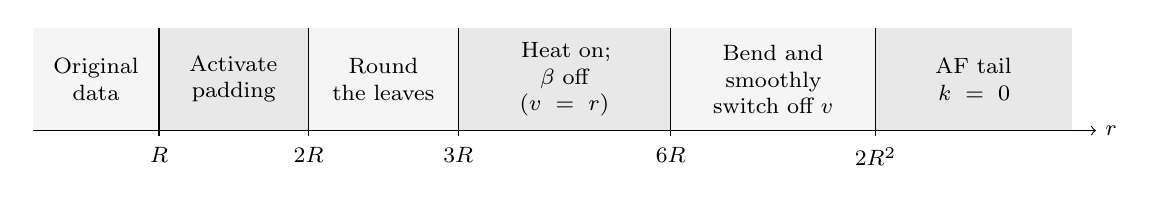
\begin{tikzpicture}[x=1cm,y=1cm,font=\footnotesize]
 \fill[black!4] (0,0) rectangle (1.6,1.3);
 \fill[black!9] (1.6,0) rectangle (3.5,1.3);
 \fill[black!4] (3.5,0) rectangle (5.4,1.3);
 \fill[black!9] (5.4,0) rectangle (8.1,1.3);
 \fill[black!4] (8.1,0) rectangle (10.7,1.3);
 \fill[black!9] (10.7,0) rectangle (13.2,1.3);
 \draw[->] (0,0) -- (13.5,0) node[right] {$r$};
 \foreach \x/\lab in {1.6/R,3.5/2R,5.4/3R,8.1/6R,10.7/2R^2}
  {\draw (\x,-0.07)--(\x,1.3);\node[below] at (\x,-0.09) {$\lab$};}
 \node[align=center,text width=1.5cm] at (0.8,0.65) {Original\\data};
 \node[align=center,text width=1.8cm] at (2.55,0.65) {Activate\\padding};
 \node[align=center,text width=1.8cm] at (4.45,0.65) {Round\\the leaves};
 \node[align=center,text width=2.5cm] at (6.75,0.65) {Heat on;\\$\beta$ off\\($v=r$)};
 \node[align=center,text width=2.4cm] at (9.4,0.65) {Bend and smoothly\\switch off $v$};
 \node[align=center,text width=2.3cm] at (11.95,0.65) {AF tail\\$k=0$};
\end{tikzpicture}
\caption{Order of the end replacement, schematically and not to scale.
The padding cutoff $w$ is one before rounding starts. The heat cutoff
$\zeta$ turns on between $4R$ and $5R$, and $\beta=0$ from $5R$ on,
while $v=r$ through $6R$. The final cutoff of $v$ occurs between $R^2$
and $2R^2$. Heat evolution and the integrable mass increase continue
on the AF tail.}\label{fig:stages}
\end{figure}

The profiles now supply a smooth metric and tensor with the required
end behavior. We must verify their dominant energy condition throughout
the transition, before using the far end to compute mass.

\emph{The exact constraints.}
Here $d=1$, $\widehat\chi=0$, $s=0$, $\eta=0$, and $U=u$.
Substituting in \eqref{eq:constraints} and
\eqref{eq:mass-identity} gives
\begin{equation}\label{eq:round-constraints}
 \begin{split}
 Q&=\frac{2u\beta}{r^3},\\
 C&=\frac vu Q+\frac{2\partial_rF}{r^2}
           -u\Delta_\gamma(u^{-1})-\frac12|\tau|_\gamma^2,\\
 Z&=\diver_\gamma\tau+(L-v/r)\mathrm d_{\Sph}\log u
                       -\tau(B_N,\cdot),
 \qquad B_N=\nabla^\gamma\log u.
 \end{split}
\end{equation}
The first formula follows as well directly from
$H=2u/r$, $p=2v/r$, and $N=u\partial_r$; the terms involving
$v'$ cancel. These are the constraint quantities of the new data,
not prescribed matter fields.

For the energy equation, direct angular differentiation yields
\begin{equation}\label{eq:laplacian-cancellation}
 \begin{split}
 u\Delta_\gamma(u^{-1})
   &=\frac{\Delta_\sigma F}{r^3u^2}
      +\frac{3|\nabla^\sigma F|_\sigma^2}{r^4u^4},\\
 \frac{2\partial_rF}{r^2}
   &=\frac{\zeta\Delta_\sigma F}{r^3A}+\frac{2}{r^{7/2}}.
 \end{split}
\end{equation}
The Laplacian coefficients cancel to the required order. Indeed,
\[
 \frac\zeta A-\frac1{u^2}
   =\frac{\zeta-1}{A}+\left(\frac1A-\frac1{u^2}\right).
\]
The first term is supported where $v=r$ and thus is $O(r^{-2})$;
the second is $O(r^{-1}A^{-2})$ by
\eqref{eq:lapse-comparison}. The angular derivatives of $F$ are
uniformly bounded. Moreover \eqref{eq:profile-derivatives} gives
\begin{equation}\label{eq:tau-acceleration-bounds}
 |\tau|_\gamma\leq\frac{C_*}{r^2\sqrt A},\qquad
 |B_N|_\gamma\leq\frac{C_*}{r^2 A},\qquad
 \mathrm d_{\Sph}\log u=-\frac{\mathrm d_{\Sph}F}{ru^2}.
\end{equation}
Finally, $Q\geq0$. Wherever $\beta\ne0$ we have $v=r$, so
$|v/u-1|=O(r^{-2})$ and $Q=O(r^{-2})$. It follows from
\eqref{eq:round-constraints}--\eqref{eq:tau-acceleration-bounds}
that
\begin{equation}\label{eq:energy-margin}
 C-Q=\frac{2}{r^{7/2}}+O(r^{-4}).
\end{equation}
All error constants here are independent of $R$.

The energy has acquired a positive margin of order $r^{-7/2}$.
To obtain DEC rather than energy positivity alone, the tangential
momentum must be smaller than that margin. Its leading term has its
own cancellation. Since
$\diver_\sigma\mathcal T=\mathrm d_{\Sph}F$, and the leafwise constant
factor $r^2$ rescales the inverse leaf metric, one has
\[
 \diver_\gamma\tau=\frac{v'-v/r}{rA}\mathrm d_{\Sph}F.
\]
Consequently its exact remaining terms are
\begin{equation}\label{eq:gradient-cancellation}
 Z=\left[
       \frac{v'-v/r}{r}\left(\frac1A-\frac1{u^2}\right)
       -\frac{\beta}{r^3u^2}
     \right]\mathrm d_{\Sph}F-\tau(B_N,\cdot).
\end{equation}
In taking its norm, $|\mathrm d_{\Sph}F|_\gamma\leq C_*/r$.
Also $|v'-v/r|\leq C_*\sqrt A/r$. Equations
\eqref{eq:lapse-comparison} and
\eqref{eq:tau-acceleration-bounds} therefore give
\begin{equation}\label{eq:momentum-error}
 |Z|_\gamma
 \leq \frac{C_*}{r^4A^{3/2}}+\frac{C_*\beta}{r^4A}
 \leq C_*r^{-4}.
\end{equation}
For sufficiently large $R$, the positive term in
\eqref{eq:energy-margin} dominates both its error and
\eqref{eq:momentum-error}, uniformly for every $r\geq3R$.
Thus
\[
 C\geq Q+|Z|_\gamma
       \geq\sqrt{Q^2+|Z|_\gamma^2},
\]
which proves the dominant energy condition. The construction used
only denominators $A$ and $u$, both bounded away from zero; in
particular, the final vanishing of $v$ causes no singularity.

\emph{Differentiated bounds and the far end.}
With $D=r\partial_r$, Equation~\eqref{eq:profile-derivatives}
gives $D^jA=O_j(A)$ and hence $D^j(A^{-1})=O_j(A^{-1})$.
Thus all fixed-order scaled derivatives of $A^{-1}$ are bounded.
Equation~\eqref{eq:heat-time}
then bounds every positive-order scaled derivative of $t$.
All positive-order scaled derivatives of $c_R$ on this region
are $O(r^{-1/2})$. The chain rule and
Lemma~\ref{lem:sphere-heat} give the asserted bounds on $F$,
including the two differentiated orders needed for the metric's
asymptotically flat decay.

For $r\geq2R^2$ one has $v=v'=\beta=0$, so $L=\tau=0$ and
$k=0$. On this tail,
\[
 t(r)=\tfrac12\log r+\kappa_R,\qquad
 c_R(r)=c_R(\infty)-2r^{-1/2}.
\]
In particular, the exponential estimate of
Lemma~\ref{lem:sphere-heat} gives the useful refinement
\begin{equation}\label{eq:tail-profile}
 F=m_B+c_R(\infty)-2r^{-1/2}+O_R(r^{-3}),
\end{equation}
where the remainder obeys the same order after any fixed number
of angular and scaled radial derivatives. The subscript allows
the decay constant in this last refinement to depend on $R$;
the uniform bounds and the dominant energy estimates above do
not have that dependence.
\end{proof}

\section{Charges, completeness and enclosing area}\label{sec:transfer}

We now finish Theorem~\ref{prop:replacement}. All estimates in this
section concern the data constructed in Sections~\ref{sec:collar}
and~\ref{sec:bending}; in particular their DEC has already been proved.
Subscripts $R$ are suppressed when they are not needed.

\subsection{The asymptotically flat output}
For each fixed sufficiently large $R$, the outer construction has
$v=\beta=0$ beyond a finite radius. Therefore $L=0$, $\tau=0$ and
$k=0$ there, and
\begin{equation}\label{eq:af-tail}
 G=(1-2F/r)^{-1}\mathrm dr^2+r^2\sigma.
\end{equation}
Lemma~\ref{lem:bending} bounds every fixed-order scaled radial and
angular derivative of $F$. In Cartesian coordinates $x=rn$ the metric
takes the form
\[
 G_{ij}=\delta_{ij}+b\,n_i n_j,
 \qquad b=(1-2F/r)^{-1}-1.
\]
Every Cartesian derivative can be expressed as
$\partial_{x_i}=r^{-1}(n_iD+X_i)$, where $D=r\partial_r$ and
$X_i$ is a smooth tangential field on the unit sphere. Repeatedly applying
this identity to $b n_i n_j$ proves
$G_{ij}-\delta_{ij}=O_j(r^{-1})$ for every fixed finite $j$.
In particular the $O_6$ metric requirement of the numerical input below
holds. The round constraint estimates
give $C=O(r^{-7/2})$ and $J=0$ on this tail. Since its volume element
is comparable to $r^2\mathrm dr\,\mathrm dA_\sigma$, the constraint
densities are integrable. The portion inside a fixed tail sphere is
compact and smooth, so integrability holds on the whole exterior.

For completeness, the ADM energy calculation allows angular dependence
of $b$. Direct differentiation, using $\partial_jn_i=(\delta_{ij}
-n_i n_j)/r$, gives
\[
 (\partial_jG_{ij}-\partial_iG_{jj})n^i=\frac{2b}{r}.
\]
The derivatives of $b$ cancel after contraction with $n$; there is no
assumption that $F$ is radial. Since $rb=2F+O(r^{-1})$, uniformly on
the sphere, \eqref{eq:adm-energy} gives
\begin{equation}\label{eq:replacement-charges}
 E_R=\lim_{r\to\infty}\avg{F(r,\cdot)}
 =m_B+c_R(\infty),\qquad P_R=0.
\end{equation}
The mean of the heat solution is constant, which proves the second
equality. The vanishing of $k$ on the tail proves $P_R=0$ directly.
The bound in \eqref{eq:mass-padding} yields
$0\leq c_R(\infty)\leq2R^{-1/2}$. Because $m_B>0$, the constructed
charges satisfy the strict inequality $E_R>|P_R|$.
These are the charges of one completed replacement, with $R$ fixed.
The constant in the refined tail estimate~\eqref{eq:tail-profile}
need not be uniform in $R$.

\subsection{A comparison for every cut}
In the balanced chart the original metric satisfies
$|g-h|_h\leq C_* r^{-3}$ for $r\geq R$. On $R\leq r\leq3R$,
Lemma~\ref{lem:collar} gives the same estimate for $G$. Beyond $3R$,
the new angular metric is exactly $r^2\sigma$ and has no shift, while
\[
 u^2=1+v^2-2F/r\leq1+r^2+2\|F\|_\infty/r.
\]
Write $M_*\geq\|F\|_\infty$ for a bound independent of $R$.
Since $0\leq v\leq r$, comparison of the radial coefficients gives
\[
 u^{-2}\geq\frac{(1+r^2)^{-1}}{1+2M_*r^{-3}}
       \geq(1-2M_*r^{-3})(1+r^2)^{-1}.
\]
The angular coefficients already agree with those of $h$. Thus
$G\geq(1-2M_*r^{-3})h$ on the whole outer region, while
$g\leq(1+C_*r^{-3})h$. Together with the collar comparison and
the identity $G=g$ on the compact interior, this gives a constant
$C_{\mathrm{met}}$ independent of $R$ such that, with
$\varepsilon_R=C_{\mathrm{met}}R^{-3}$,
\begin{equation}\label{eq:metric-comparison}
 G_R\geq(1-\varepsilon_R)g\quad\hbox{on all of }\Omega.
\end{equation}
We increase $R$ once so that $0\leq\varepsilon_R<1$.

This also proves completeness, including the boundary. A $G_R$-Cauchy
sequence is $g$-Cauchy by \eqref{eq:metric-comparison}, and hence has a
limit in $\Omega$. The smooth positive metrics induce the same local
topology, so it converges in $G_R$ as well. The manifold, its boundary,
and its single end have not changed. Compact truncations remain compact
after the balancing chart change because old and new radii are
comparable sufficiently far out.

On the tangent plane of any smooth cut, the two relative eigenvalues
of $G_R$ with respect to $g$ are at least $1-\varepsilon_R$. Its area
element is therefore at least $(1-\varepsilon_R)$ times the original
area element. The admissible cuts are the same geometric surfaces for
the two metrics, with the same filled-side convention. Taking the
infimum over \emph{all} such surfaces gives
\begin{equation}\label{eq:area-comparison}
 A_{\min,G_R}(S)\geq(1-\varepsilon_R)A_{\min,g}(S).
\end{equation}
This includes cuts coinciding with the obstacle $S$. It uses neither
existence of a minimizing cut nor any identification of its area with
the area of $S$. Equations~\eqref{eq:replacement-charges}--
\eqref{eq:area-comparison}, together with the smooth DEC construction,
prove Theorem~\ref{prop:replacement}.

\subsection{The numerical input and the Bondi bound}\label{sec:companion-input}
The replacements now have the geometric properties needed for the
numerical step. We use the dimension-three case of the companion
\cite[Definitions~1.1--1.2 and Theorem~1.3]{NumericalPenrose}, stated
here with our physical constraint normalization.

\begin{theorem}[Asymptotically flat numerical input]
\label{ass:af}
Let $(X,q,k)$ be a smooth connected orientable three-dimensional
exterior, complete including its nonempty compact smooth boundary,
with exactly one asymptotically flat coordinate end and compact
complement. Suppose that, in Cartesian coordinates, for some
$1/2<a<1$,
\[
 q_{ij}-\delta_{ij}=O_6(r^{-a}),\qquad
 k_{ij}=O_5(r^{-1-a}).
\]
Use the constraints \eqref{eq:constraints-definition} and ADM
normalizations \eqref{eq:adm-energy}--\eqref{eq:adm-momentum}.
Assume DEC, integrability of $\mu$ and $|J|_q$, finite ADM limits,
$E>|P|$, and $A_{\min,q}(\partial X)>0$. If every boundary component
satisfies $\theta_+\leq0$ with normal into $X$, then
\[
 \sqrt{E^2-|P|^2}\geq
 \sqrt{\frac{A_{\min,q}(\partial X)}{16\pi}}.
\]
The full cut class is that of \eqref{eq:area-definition}, including
disconnected cuts and partial or whole coincidence with the boundary.
No extension across the boundary, outermostness, outer
area-minimization or attainment of the infimum is assumed.
\end{theorem}

To identify this statement with the cited theorem, its densities satisfy
\[
 2\mu_{\mathrm N}=R+(\tr k)^2-|k|^2,\qquad
 J_{\mathrm N}=\diver(k-(\tr k)q).
\]
Thus $\mu_{\mathrm N}=8\pi\mu$ and $J_{\mathrm N}=8\pi J$;
the common positive factor preserves DEC and integrability. At
dimension three its ADM factors are
$[2(n-1)\omega_{n-1}]^{-1}=1/(16\pi)$ and
$[(n-1)\omega_{n-1}]^{-1}=1/(8\pi)$, so the charges are unchanged.
Its Definition~1.2 takes the full intrinsic boundary of the connected
closed end-containing outer domain, including every component and
all contact with the original boundary. This is precisely the cut
class in \eqref{eq:area-definition}.

\begin{proof}[Proof of Corollary~\ref{cor:cks-inequality}]
Fix a sufficiently large $R$. The data $(G_R,k_R)$ have the same
connected orientable manifold, compact boundary and single end as the
original data. Their completeness follows from
\eqref{eq:metric-comparison}. Both tensors agree with $(g,K)$ on a
neighborhood of $S$, so its normal, mean curvature, tangential tensor
trace and weak future trapping are unchanged. The construction proves
DEC and integrable constraint densities. On the completed tail,
$G_R-\delta=O_6(r^{-1})$ and $k_R=0$, which give the required
differentiated rates with $a=3/4$. Equation~\eqref{eq:area-comparison}
and the assumed positivity of $A_{\min,g}(S)$ give
$A_{\min,G_R}(S)>0$. Finally,
\eqref{eq:replacement-charges} gives finite charges with
$E_R=m_B+c_R(\infty)>0=|P_R|$.

Thus every hypothesis of the companion's numerical theorem, in the
form of Theorem~\ref{ass:af}, holds for this fixed replacement.
Using the comparison of all cuts gives
\begin{equation}\label{eq:finite-numerical}
 m_B+c_R(\infty)
 \geq\sqrt{\frac{A_{\min,G_R}(S)}{16\pi}}
 \geq\sqrt{\frac{(1-\varepsilon_R)A_{\min,g}(S)}{16\pi}}.
\end{equation}
Only now let $R\to\infty$, using $0\leq c_R(\infty)\leq2R^{-1/2}$
and $\varepsilon_R\to0$. This proves \eqref{eq:main}. The examples
in Section~\ref{sec:sharpness} establish sharpness.
\end{proof}

There are two successive infinities in this proof. Radial infinity
defines the ADM charges of one completed replacement. The replacement
radius tends to infinity only after its numerical inequality has
been proved. No convergence of comparison metrics or minimizing cuts
is required, and the constant in $O_R(r^{-3})$ need not be uniform in
the replacement radius.

\begin{remark}[The weaker-decay numerical theorem]
The companion also proves the same inequality directly under
$q-\delta=O_2(r^{-a})$, $k=O_1(r^{-1-a})$, $a>1/2$, for the same
smooth one-ended exterior and full cut class, with physical constraint
densities, integrable DEC, finite timelike charges, and weakly future
trapped boundary \cite[Definition~7.1 and Theorem~7.2]{NumericalPenrose}.
That theorem does not assume positivity of the enclosing infimum.
It gives another numerical input for our replacements; its weaker
original-data hypotheses are a separate result, not a consequence of
changing the exponent in Theorem~\ref{ass:af}.
\end{remark}

\paragraph{Dependence on the numerical input.}\label{sec:conditional}
The proof uses the companion only through the displayed asymptotically
flat inequality. More generally, this inequality is the sole numerical
input needed for the same argument to give the Bondi bound for every weakly future trapped,
possibly disconnected boundary under the other hypotheses of
Corollary~\ref{cor:cks-inequality}. In particular, it applies when $S$
is connected and marginal, and the open exterior contains no compact
smooth embedded two-sided separating union of closed future or past
apparent horizons, allowing either sign on each component. These
additional horizon conditions are not needed for the transfer.
The Schwarzschild examples below satisfy them and attain the bound
at every positive mass.

The inequality alone does not classify equality for the original data:
the construction need not preserve an equality case at finite $R$.
A classification, or an extension to weaker null-infinity expansions,
would require a further argument.

\section{Schwarzschild equality examples}\label{sec:sharpness}

The radial model gives equality examples once its inner endpoint is
placed on the future Schwarzschild horizon. We verify their geometry
at that endpoint, their CKS charges at infinity, and the area of every
enclosing cut. The examples also exclude every closed interior apparent
horizon of either time orientation.

Fix $m>0$ and let $\Omega=[2m,\infty)\times\Sph$. Choose a smooth
function $v(r)$ equal to $-1$ near $2m$ and to $r$ for all sufficiently
large $r$. Define
\begin{equation}\label{eq:schwarzschild-data}
\begin{gathered}
 u^2=1-\frac{2m}{r}+v^2,\qquad
 G=u^{-2}\mathrm dr^2+r^2\sigma,\qquad N=u\partial_r,\\
 k(N,N)=v',\qquad k(N,\cdot)|_{T\Sph}=0,
 \qquad k|_{T\Sph\times T\Sph}=(v/r)r^2\sigma.
\end{gathered}
\end{equation}
The function $u$ is strictly positive at the boundary and throughout
the exterior, including any interior zero of $v$. Thus these are smooth
data up to $S=\{2m\}\times\Sph$. At infinity $u\sim r$, so the radial
length $\int^\infty u^{-1}\mathrm dr$ diverges logarithmically.
Together with compactness of finite truncations, this proves completeness.
Substitution in \eqref{eq:round-constraints}, or directly in
\eqref{eq:constraints}, gives $C=Q=Z=0$: here $F=m$, $\eta=\tau=0$,
and $L=v'$. In particular the data are vacuum.

\subsection{Spacetime realization and the future boundary}
To verify their Schwarzschild interpretation and sign, write
$h_m=1-2m/r$. On $r>2m$ the Schwarzschild metric is
\[
 \overline g=-h_m\mathrm dt_s^2+h_m^{-1}\mathrm dr^2+r^2\sigma.
\]
Take a graph $t_s=t_s(r)$ with
\[
 t_s'=\frac{v}{h_m u}.
\]
Its induced radial metric coefficient is $u^{-2}$. The future unit
normal and outward radial unit tangent have $(t_s,r)$-components
\[
 n_{\mathrm{future}}=(u/h_m,v),\qquad e_r=(v/h_m,u).
\]
The tangential sphere component of its second fundamental form is
$(v/r)r^2\sigma$. The radial component of
$\overline\nabla_{e_r}n_{\mathrm{future}}$ is $uv'$: the connection
terms from
$\overline\Gamma^r_{t_st_s}=h_mh_m'/2$ and
$\overline\Gamma^r_{rr}=-h_m'/(2h_m)$ cancel. Orthogonality to the
future normal then gives $k(e_r,e_r)=v'$, with mixed component zero.
This proves exactly the convention used in \eqref{eq:schwarzschild-data}.

In advanced time $w=t_s+\int h_m^{-1}\mathrm dr$, the spacetime metric
is regular at the future horizon. Along the graph,
\[
 \frac{\mathrm dw}{\mathrm dr}
 =\frac{u+v}{h_m u}=\frac1{u(u-v)}.
\]
The latter expression is smooth at $r=2m$ because $v=-1$ there and
$u=1$. Thus the slice extends smoothly to the future horizon, not to
the opposite horizon with the wrong expansion sign. At $S$,
\[
 \theta_+(S)=\frac{2(u+v)}r=0.
\]

For large $r$ we have $v=r$, $v'=1$, and hence $k=G$. Moreover
\[
 G-h=\left(\frac1{1+r^2-2m/r}-\frac1{1+r^2}\right)\mathrm dr^2
 =\left(\frac{2m}{r^5}+O_3(r^{-7})\right)\mathrm dr^2.
\]
The CKS expansion holds with $m^r=2m$ and $m^g=m^K=0$.
Consequently $M=4m$, $E_B=m$, $P_B=0$, and $m_B=m>0$.

\subsection{No further horizon and the exact area infimum}
Every interior coordinate sphere satisfies
\begin{equation}\label{eq:sphere-barrier}
 H=\frac{2u}{r}>\frac{2|v|}{r}
 =\bigl|\tr_{\mathrm{sphere}}k\bigr|,
\end{equation}
because $u^2-v^2=1-2m/r>0$. This also rules out nonround apparent
horizons. Indeed, let $T$ be any compact closed embedded two-sided
surface in the interior, and let $x$ be a maximum of $r|_T$. The
tangent plane at $x$ is tangent to the coordinate sphere. Orient $T$
locally by the radial outward normal. The surface Hessian identity
and $\Delta_T r(x)\leq0$ give
\[
 0\geq\Delta_T r(x)
 =\tr_{T_xT}\nabla_G^2r-uH_T(x)
 =u\left(\frac{2u}{r}-H_T(x)\right).
\]
Thus $H_T(x)\geq2u/r>|\tr_{T_xT}k|$. Reversing the orientation
changes $H_T$ only by sign, so neither $\theta_+=0$ nor $\theta_-=0$
can hold on $T$. The argument applies to every component of a
separating union of closed surfaces, even if different components
are assigned different horizon signs.

Finally let $\pi:\Omega\to S$ be radial projection. Since $r\geq2m$
and the metric is $u^{-2}\mathrm dr^2+r^2\sigma$, this map is length
nonincreasing. A radial ray from $S$ to infinity starts on the filled
inner side, or on the cut itself, and eventually enters the retained
outer domain. It therefore meets every enclosing cut $\Gamma$;
at a point of boundary coincidence the initial point is already an
intersection. Thus $\pi|_\Gamma$ is
surjective. The area formula, with absolute two-dimensional Jacobian
at most one, implies
\[
 \operatorname{Area}_G(\Gamma)\geq\operatorname{Area}_G(S)
 =16\pi m^2.
\]
As $S$ itself is an allowed cut,
$A_{\min,G}(S)=16\pi m^2>0$. Equality in \eqref{eq:main} follows.
These examples prove the sharpness assertion in
Corollary~\ref{cor:cks-inequality}, including its connected marginal
specialization.

\begin{thebibliography}{99}
\addcontentsline{toc}{section}{References}

\bibitem{Alexakis}
S.~Alexakis,
\emph{The Penrose inequality on perturbations of the Schwarzschild exterior},
preprint (2015),
\href{https://arxiv.org/abs/1506.06400v1}{arXiv:1506.06400v1}.

\bibitem{ABKK}
B.~Allen, E.~Bryden, D.~Kazaras, and M.~Khuri,
\emph{Proof of the spacetime Penrose inequality with suboptimal constant in the asymptotically flat and asymptotically hyperboloidal regimes},
preprint (2025),
\href{https://arxiv.org/abs/2504.10641v1}{arXiv:2504.10641v1}.

\bibitem{Bartnik}
R.~Bartnik,
\emph{Quasi-spherical metrics and prescribed scalar curvature},
J. Differential Geom. \textbf{37} (1993), no.~1, 31--71.
\href{https://doi.org/10.4310/jdg/1214453422}{doi:10.4310/jdg/1214453422}.

\bibitem{BartnikICM}
R.~Bartnik,
\emph{Mass and 3-metrics of non-negative scalar curvature},
in \emph{Proceedings of the International Congress of Mathematicians,
Beijing 2002}, Vol.~II, 231--240.
\href{https://arxiv.org/abs/math/0304259v1}{arXiv:math/0304259v1}.

\bibitem{BenDov}
I.~Ben-Dov,
\emph{The Penrose inequality and apparent horizons},
Phys. Rev. D \textbf{70} (2004), 124031.
\href{https://doi.org/10.1103/PhysRevD.70.124031}{DOI}.
Locators refer to
\href{https://arxiv.org/abs/gr-qc/0408066v2}{arXiv:gr-qc/0408066v2}.

\bibitem{Bray}
H.~L.~Bray,
\emph{Proof of the Riemannian Penrose inequality using the positive mass theorem},
J. Differential Geom. \textbf{59} (2001), no.~2, 177--267.
\href{https://doi.org/10.4310/jdg/1090349428}{doi:10.4310/jdg/1090349428}.

\bibitem{CKS}
Y.~S.~Cha, M.~Khuri, and A.~Sakovich,
\emph{Reduction arguments for geometric inequalities associated with asymptotically hyperboloidal slices},
Class. Quantum Grav. \textbf{33} (2016), no.~3, 035009.
\href{https://doi.org/10.1088/0264-9381/33/3/035009}{doi:10.1088/0264-9381/33/3/035009};
\href{https://arxiv.org/abs/1509.06255v2}{arXiv:1509.06255v2}.

\bibitem{CWY}
P.-N.~Chen, M.-T.~Wang, and S.-T.~Yau,
\emph{Conserved quantities on asymptotically hyperbolic initial data sets},
Adv. Theor. Math. Phys. \textbf{20} (2016), no.~6, 1337--1375.
\href{https://doi.org/10.4310/ATMP.2016.v20.n6.a2}{DOI};
\href{https://arxiv.org/abs/1409.1812v1}{arXiv:1409.1812v1}.

\bibitem{ChruscielDelay}
P.~T.~Chru\'sciel and E.~Delay,
\emph{The hyperbolic positive energy theorem},
preprint (2019), revised 2 April 2026.
Locators refer to
\href{https://arxiv.org/abs/1901.05263v3}{arXiv:1901.05263v3}.

\bibitem{CJL}
P.~T.~Chru\'sciel, J.~Jezierski, and S.~\L{}\k{e}ski,
\emph{The Trautman--Bondi mass of hyperboloidal initial data sets},
Adv. Theor. Math. Phys. \textbf{8} (2004), no.~1, 83--139.
\href{https://doi.org/10.4310/ATMP.2004.v8.n1.a2}{DOI}.
Locators refer to
\href{https://arxiv.org/abs/gr-qc/0307109v2}{arXiv:gr-qc/0307109v2}.

\bibitem{CorvinoHuang}
J.~Corvino and L.-H.~Huang,
\emph{Localized deformation for initial data sets with the dominant energy condition},
Calc. Var. Partial Differential Equations \textbf{59} (2020), article~42.
\href{https://doi.org/10.1007/s00526-019-1679-9}{DOI}.
Locators refer to
\href{https://arxiv.org/abs/1606.03078v2}{arXiv:1606.03078v2}.

\bibitem{Ellithy}
A.~Ellithy,
\emph{The spacetime Penrose inequality under a quasi final state hypothesis},
preprint (2026),
\href{https://arxiv.org/abs/2605.18730v1}{arXiv:2605.18730v1}.

\bibitem{HI}
G.~Huisken and T.~Ilmanen,
\emph{The inverse mean curvature flow and the Riemannian Penrose inequality},
J. Differential Geom. \textbf{59} (2001), no.~3, 353--437.
\href{https://doi.org/10.4310/jdg/1090349447}{doi:10.4310/jdg/1090349447}.

\bibitem{MarsSoria}
M.~Mars and A.~Soria,
\emph{On the Penrose inequality along null hypersurfaces},
Class. Quantum Grav. \textbf{33} (2016), no.~11, 115019.
\href{https://doi.org/10.1088/0264-9381/33/11/115019}{DOI}.
Locators refer to
\href{https://arxiv.org/abs/1511.06242v1}{arXiv:1511.06242v1}.

\bibitem{NumericalPenrose}
OpenAI,
\emph{The spacetime Penrose inequality and enclosing area},
OpenAI Math Release preprint
\href{https://github.com/openai/math/blob/main/preprints/The-spacetime-Penrose-inequality-and-enclosing-area-September-27-2026/paper.pdf}{OAI:The-spacetime-Penrose-inequality-and-enclosing-area-September-27-2026},
2026.

\bibitem{Penrose}
R.~Penrose,
\emph{Naked singularities},
Ann. New York Acad. Sci. \textbf{224} (1973), 125--134.
\href{https://doi.org/10.1111/j.1749-6632.1973.tb41447.x}{DOI}.

\bibitem{Sakovich}
A.~Sakovich,
\emph{The Jang equation and the positive mass theorem in the asymptotically hyperbolic setting},
Comm. Math. Phys. \textbf{386} (2021), no.~2, 903--973.
\href{https://doi.org/10.1007/s00220-021-04083-1}{doi:10.1007/s00220-021-04083-1};
\href{https://arxiv.org/abs/2003.07762v2}{arXiv:2003.07762v2}.

\end{thebibliography}

\end{document}
